\documentclass{article}

% if you need to pass options to natbib, use, e.g.: \PassOptionsToPackage{numbers, compress}{natbib}
% before loading nips_2016
% to avoid loading the natbib package, add option nonatbib: \usepackage[nonatbib]{nips_2016}

\PassOptionsToPackage{numbers, compress}{natbib}
\usepackage{nips_2016}
% to compile a camera-ready version, add the [final] option, e.g.:
%\usepackage[final]{nips_2016}

\usepackage[utf8]{inputenc} % allow utf-8 input
\usepackage[T1]{fontenc}    % use 8-bit T1 fonts
\usepackage{hyperref}       % hyperlinks
\usepackage{url}            % simple URL typesetting
\usepackage{booktabs}       % professional-quality tables
\usepackage{amsfonts}       % blackboard math symbols
\usepackage{amssymb}       % blackboard math symbols
\usepackage{nicefrac}       % compact symbols for 1/2, etc.
\usepackage{microtype}      % microtypography
\usepackage{graphicx}
\usepackage{caption}
\usepackage{subcaption}

\usepackage{amsmath,amsthm,color,graphicx,verbatim,listings,enumitem}
\usepackage[]{algorithm2e}
\graphicspath{{figures/}}

\lstset{
numbers=left, 
numberstyle=\small, 
numbersep=8pt, 
frame = single, 
language=matlab, 
framexleftmargin=20pt}

\newtheorem{lemma}{Lemma}
\newtheorem{theorem}{Theorem}

\title{An Efficient Minibatch Acceptance Test for Metropolis-Hastings}

% The \author macro works with any number of authors. There are two commands used to separate the
% names and addresses of multiple authors: \And and \AND.
% Using \And between authors leaves it to LaTeX to determine where to break the lines. Using \AND
% forces a line break at that point. So, if LaTeX puts 3 of 4 authors names on the first line, and
% the last on the second line, try using \AND instead of \And before the third author name.

%%  David S.~Hippocampus\thanks{Use footnote for providing further
%%    information about author (webpage, alternative
%%    address)---\emph{not} for acknowledging funding agencies.} \\
%%  Department of Computer Science\\
%%  Cranberry-Lemon University\\
%%  Pittsburgh, PA 15213 \\
%%  \texttt{hippo@cs.cranberry-lemon.edu} \\


\author{
  Haoyu Chen \\
  Department of Computer Science \\
  University of California, Berkeley \\
  \texttt{haoyuchen@berkeley.edu}
  \And
  Daniel Seita \\
  Department of Computer Science \\
  University of California, Berkeley \\
  \texttt{seita@berkeley.edu}
  \And
  Xinlei Pan \\
  Department of Bioengineering \\
  University of California, Berkeley \\
  \texttt{xinleipan@berkeley.edu}
  \And 
  Biye Jiang \\
  Department of Computer Science \\
  University of California, Berkeley \\
  \texttt{bjiang@berkeley.edu}
  \And
  John Canny \\
  Department of Computer Science \\
  University of California, Berkeley \\
  \texttt{canny@berkeley.edu}
}

\begin{document}
\maketitle

\begin{abstract}
Markov chain Monte Carlo (MCMC) methods have many applications in
machine learning. We are particularly interested in their application
to modeling very large datasets, where it is impractical to perform
Metropolis-Hastings tests on the full data. Previous work on reducing
the cost of Metropolis-Hastings tests yield variable data reductions
and in the worst case require the entire dataset.  Here we present a
simple test which requires constant size minibatches if an auxiliary
condition is met. We describe several cases under which this condition
can be satisfied. Our new test is naturally tolerant of ``noisy''
estimates of the transition probability ratio. To achieve this, we
replace the classical Metropolis-Hastings acceptance test with a
smooth acceptance function which is a sigmoid (logistic)
function of the log likelihood ratio.
The resulting test can be combined with minibatch proposals to yield
updates with the same complexity as a simple SGD update. In this paper
we derive the test, discuss its implementation, and present several
experiments.
\end{abstract}



\section{Introduction}\label{sec:introduction}

Markov chain Monte Carlo (MCMC) sampling is a powerful method for
computation on intractable distributions. We are interested primarily
in large dataset applications, where the goal is to sample a posterior
distribution $p(\theta \mid x_1, \ldots, x_N)$ of parameter $\theta$,
and where the number of data instances $N$ is large.  The
Metroplis-Hastings method (M-H) generates sample candidates from a
proposal distribution $q$ which is in general different from the
target distribution $p$, and decides whether to accept or reject them
based on an acceptance test. The acceptance test is usually a
Metropolis test~\cite{Metropolis1953,hastings70}. Conventional
Metropolis-Hastings requires all $N$ data instances to generate one
posterior sample.

Many state-of-the-art machine learning methods, and deep learning in
particular, are based on minibatch updates (such as SGD) to a model.
Minibatch updates produce many improvements to the model for each pass
over the dataset, and have high sample efficiency. They also
map very well onto hardware such as GPUs. In contrast, M-H requires
calculations over the full dataset to produce a new sample.  Recent
results from~\cite{cutting_mh_2014,icml2014c1_bardenet14} perform
approximate (bounded error) acceptance tests using subsets
(minibatches) of the full dataset. The tests depend on minibatch
statistics, and on the value of an additional random variable $u$. The
amount of data consumed for each test varies significantly from one
minibatch to the next, and depends on the current sample, the proposed
sample, and on the random variable $u$. By contrast,
\cite{conf/uai/MaclaurinA14} performs exact tests but requires a lower
bound on parameter distribution across its domain. The amount of data
reduction depends on the accuracy of this bound, and such bounds are
only available for relatively simple distributions.

Here we derive a new test which incorporates the variability in
minibatch statistics as {\em a natural part of the test}. Because of
this, the amount of data required for each test is fixed with high
probability and in expected value. Our test requires a bound on the
(relative) variance of the log acceptance probability. This variance
is small when the proposal distribution is efficient, that is when samples
diffuse at an optimal rate.

The variance of the log acceptance probability can be controlled in
three ways, and these allow the test to be applied to modest-sized
minibatches. The first two allow the test to be applied when the
minibatch size is fixed a-priori.

\begin{itemize}
  
\item Increase the temperature of the target distribution. Log likelihoods
  scale as $1/T$, and so the variance of the likelihood ratio will
  vary as $1/T^2$.

\item For continuous probability distributions, reduce the proposal
  step size and variance (for stochastic proposals). 

\item Increase the minibatch size. Relative variance scales as $1/k$ vs the
  minibatch size $k$. Increased minibatch size also reduces the error of
  the test. 

\end{itemize}

The contributions of this paper are as follows:

\begin{itemize}
\item We develop a new, more efficient (in samples per test) minibatch acceptance test which incorporates
online  estimates of its error probability.
\item We analyze the test for accuracy and speed.
\item We compared performance of our new test and prior approaches on several datasets. We demonstrate the test is several orders
  of magnitude more efficient than prior work measured as data consumed per test, and that it does not suffer
  from long-tailed data requirements (up to the dataset size). 
\end{itemize}




\section{Preliminaries and Related Work}\label{sec:related_work}

In the Metropolis-Hastings method~\cite{gilks1996markov,brooks2011handbook}, a difficult-to-compute
probability distribution $p(\theta)$ is sampled using a Markov chain $\theta_1,\ldots,\theta_n$. The 
sample $\theta_{t+1}$ at time $t+1$ is generated using a candidate $\theta'$ from a (simpler) proposal
distribution $q(\theta'\mid \theta_t)$, filtered by an acceptance test. The acceptance test is usually
a Metropolis test. The Metropolis test has acceptance probability:
\begin{equation}\label{eq:traditional}
\alpha(\theta_t,\theta') = \min\left\{ 1, \frac{p(\theta')q(\theta_t \mid \theta')}{p(\theta_t)q(\theta' \mid \theta_t)}
\right\}
\end{equation}
and with probability $\alpha(\theta_t,\theta')$, we accept $\theta'$
and set $\theta_{t+1} = \theta'$, otherwise set
$\theta_{t+1}=\theta_t$.  The test is often implemented with an
auxiliary random variable $u \sim \mathcal{U}(0,1)$ with a comparison $u < \alpha(\theta_t,\theta')$.
For notational simplicity, from now on we will drop the subscript $t$ for the current sample $\theta_t$ and
denote is simply as $\theta$. 


The acceptance test guarantees detailed balance, which means
\begin{equation}\label{detailed_balance1}
  p(\theta)p(\theta,\theta') = p(\theta')p(\theta',\theta)
\end{equation}
where $p(\theta,\theta')$ is the probability of a transition from state $\theta$ to $\theta'$. Here
$p(\theta,\theta') = q(\theta'\mid\theta)\alpha(\theta,\theta')$ so the detailed balance equation becomes
\begin{equation}\label{detailed_balance2}
  p(\theta)q(\theta'\mid\theta)\alpha(\theta,\theta') = p(\theta')q(\theta\mid\theta')\alpha(\theta',\theta)
\end{equation}
The detailed balance condition, together with ergodicity, guarantee that the
Markov chain has a unique stationary distribution $\pi(\theta) = p(\theta)$.

For Bayesian inference, we would like to sample from a parameter distribution for $\theta$ based on some
observed data $x_1,\ldots,x_N$. i.e. we want to sample from 
$p(\theta \mid x_1, \ldots, x_N)$. The acceptance probability is now:
\begin{equation}
\alpha(\theta,\theta') = 
\min\left\{ 1, \frac{p_0(\theta')\prod_{i=1}^N p(x_i \mid \theta')q(\theta \mid
\theta')}{p_0(\theta)\prod_{i=1}^N p(x_i \mid \theta)q(\theta' \mid\theta)} \right\},
\end{equation}
where $p_0(\theta)$ is a prior, and $p(x_i \mid \theta)$ are the
probabilities of the observations. Computing samples this way requires
the use of all $N$ training data points, but this is very expensive
for large datasets. To address this challenge,~\cite{cutting_mh_2014,icml2014c1_bardenet14} perform
approximate Metropolis-Hasting tests using sequential hypothesis
testing. During each iteration, they start with a small minibatch of
data and test the hypothesis that the sample $\theta'$ based on an
approximate version of the test $u < \alpha(\theta,\theta')$. If the
approximate test cannot make a decision with sufficient confidence,
then the minibatch size is increased and the test repeats. This
process continues until a decision. The bounds depend on either a
asymptotic central limit theorem \cite{cutting_mh_2014} or a
concentration bound \cite{icml2014c1_bardenet14}, the latter requiring
direct bounds on the log likelihood ratio.  The problem with both
methods is the expense of resolving small differences.  In the worst
case, all $N$ data points may be needed, and as we show next this
worst case can occur about $\Omega(N)$ times during the performance of
$N$ tests.

Following ~\cite{icml2014c1_bardenet14}, we write the test $u < \alpha(\theta,\theta')$ in
the equivalent form $\Lambda(\theta,\theta') > \psi(u,\theta,\theta')$ where
\begin{equation}
\Lambda(\theta,\theta') = \frac{1}{N}\sum_{i=1}^N \log\left(\frac{p(x_i|\theta')}{p(x_i|\theta)}\right)  
\hspace{0.2in} {\rm and} \hspace{0.2in}
\psi(u,\theta,\theta') = \frac{1}{N}\log\left(u\frac{q(\theta'|\theta)p_0(\theta)}{q(\theta|\theta')p_0(\theta')}\right)
\end{equation}

To reduce computational effort, an unbiased estimate of $\Lambda(\theta,\theta')$
based on a minibatch can be used:

\begin{equation}
\Lambda^*(\theta,\theta') = \frac{1}{b}\sum_{i=1}^b \log\left(\frac{p(x_i|\theta')}{p(x_i|\theta)}\right)  
\end{equation}

The minibatch should contain randomly selected samples, and
by the central limit theorem, we expect $\Lambda^*(\theta,\theta')$ to be approximately
Normal. 
The acceptance test then becomes a statistical test of the hypothesis
that $\Lambda(\theta,\theta') > \psi(u,\theta,\theta')$ by
establishing that $\Lambda^*(\theta,\theta')$ is substantially larger
than $\psi(u,\theta,\theta')$.  In ~\cite{cutting_mh_2014} an
asymptotic central limit argument was used to derive this gap, while
in \cite{icml2014c1_bardenet14} a concentration bound was used. In
both cases, the resulting tests were shown to give useful reductions
in number of samples required over using the full dataset. But no
worst-case bounds were given on average number of samples needed.

We next show that for some simple distributions, the lower
bound of average number of data instances consumed for one iteration of
~\cite{cutting_mh_2014} and ~\cite{icml2014c1_bardenet14} is
$\Omega(N)$, where $N$ is the number of data points.

\subsection{An Example}
Consider a simple model where samples $x_i$ for $i=1,\ldots,N$ are
drawn from a Normal distribution $\mathcal{N}(\theta,1)$ where
$\theta=0.5$, and with a uniform prior on $\theta$. The log likelihood ratio is
\begin{equation}
\Lambda^*(\theta,\theta') =  \frac{1}{b}\sum_{i=1}^b \log\frac{p(x_i|\theta')}{p(x_i|\theta)}=
  %%\frac{1}{2}\left( (x_i-\theta')^2 - (x_i - \theta)^2\right) =
  (\theta'-\theta)\left(\frac{1}{b}\sum_{i=1}^b x_i-\theta-\frac{\theta'-\theta}{2}\right)
\end{equation}
which is normally distributed over selection of the Normal samples $x_i$.
Since the $x_i$ have unit variance, their mean has variance $1/b$, and the variance $\sigma^2(\Lambda^*)$
of $\Lambda^*(\theta,\theta')$ is $(\theta'-\theta)^2/b$. In order to pass
a hypothesis test that $\Lambda > \psi$, we will need to establish a
large enough gap (several $\sigma(\Lambda^*)$) between $\Lambda^*(\theta',\theta)$
and $\psi(u,\theta',\theta)$.

We would like to sample from the posterior distribution of $\theta$
which is a normal distribution centered on the sample mean, and with
variance $1/N$.  The target distribution is therefore
$\mathcal{N}(\mu,1/N)$ where $\mu$ is the sample mean.  An efficient
proposal distribution has the same variance as the target distribution
$\mathcal{N}(\theta'-\theta,1/N)$, so we take $q(\theta'\mid\theta) =
\phi((\theta'-\theta)N)$, where $\phi(x)$ is the Normal density
function with zero mean and unit variance. This proposal is symmetric
$q(\theta',\theta)=q(\theta,\theta')$, and we assumed uniform
prior for $\theta$, so $\psi(u,\theta',\theta)$ reduces to $1/N\log
u$.

\begin{lemma}\label{lem:efficienty_cutting}
  For the model above, there
  exists a fixed (independent of $N$) constant $c$ such that with probability $ \geq c$ over the joint
  distribution of $(\theta, \theta', u)$, the
  tests from \cite{icml2014c1_bardenet14} and \cite{cutting_mh_2014} consume all $N$ samples. 
\end{lemma}

\begin{proof} Assume $(\theta' - \theta) \in \pm\frac{1}{\sqrt{N}}[0.5,1]$ and
  $\theta -0.5 \in \pm\frac{1}{\sqrt{N}}[0.5,1]$ with matching sign. These events
  occur with probability $p_0=2*(\Phi(1)-\Phi(0.5)) = 0.2997$ and $p_1=(\Phi(1)-\Phi(0.5))=0.14988$ respectively,
  and guarantee that $\Lambda^*(\theta',\theta)$ is negative, which guarantees that we can find
  a $u$ so that $\psi(u,\theta',\theta)$ equals the expected value of $\Lambda^*(\theta',\theta)$.
  Specifically, choose $u_0$
  to satisfy
  \begin{equation}
    \log u_0 = N(\Lambda^*(\theta',\theta)-\psi(1,\theta',\theta))
  \end{equation}
  which evaluates to 
  \begin{equation}
    \log u_0 = -N(\theta'-\theta)\left(\theta-0.5+\frac{\theta'-\theta}{2}\right) 
  \end{equation}
  and rewrite the test now as
  \begin{equation}
    \frac{1}{b}\sum_{i=1}^b x_i-\left(\theta+\frac{\theta'-\theta}{2} + \frac{\log u_0}{N(\theta'-\theta)}\right)
    \hspace{0.1in} \not\approx \hspace{0.1in} 0
  \end{equation}
  where $\not\approx$ means ``significantly different from'' under the distribution over samples of $x_i$. 
  The above choice of $u_0$ ensures that the terms in parenthesis above sum to 0.5. Since the $x_i$ have mean 0.5, the
  test will never correctly succeed.

  Furthermore, if we sample values of $u$ near enough to $u_0$, the terms in parenthesis will not be sufficiently different
  from 0.5 to allow the test to succeed. 
  
 The choices above for $\theta$ and $\theta'$ guarantee that
  \begin{equation}
    \log u_0 \in -[0.5,1][0.75,1.5] = -[0.375,1.5]
        \end{equation}
and consider the range of $u$ values
  \begin{equation}
    \log u \in \log u_0 + [-0.5,0.375]
  \end{equation}
  the size of the range in $u$ is at least $\exp([-2,-1.125]) = [0082,0.286]$ and occurs
  with probability at least $p_2=0.2044$. With $u$ in this range, we rewrite the test as:
  \begin{equation}
    \frac{1}{b}\sum_{i=1}^b x_i-0.5 \hspace{0.1in} \not\approx \hspace{0.1in} \frac{\log u/u_0}{N(\theta'-\theta)}
  \end{equation}
  so that the LHS has expected value zero.  Given our choice of intervals for the variables, the RHS is in the range $1/\sqrt{N}[-1,0.75]$.
  The standard deviation of the LHS given the interval constraints is at least $0.5/\sqrt{b}$. And
  so the gap between LHS and RHS is at most $2\sqrt{b/N}$ standard deviations. 


  The samples $\theta$, $(\theta'-\theta)$
  and $u$ are drawn independently and so the probability of the conjunction of these events is
  $c = p_0 p_1 p_2 = 0.009$.
\end{proof}

Similar results can be proved for other distributions and proposals, by identifying
regions in product space $(\theta,\theta'-\theta,u)$ such that the hypothesis test
needs to separate nearly-equal values. 

It follows that the accelerated M-H tests in \cite{icml2014c1_bardenet14} and
\cite{cutting_mh_2014} require at least a constant fraction $\geq c$
in the amount of data consumed per test, compared to full-dataset tests.
i.e. their speed-up is at most $1/c$.

\subsection{MCMC Posterior Inference}
There is a separate line of MCMC work drawing principles from
statistical physics. By viewing random variables as particles in a
system, one can apply Hamiltonian Monte Carlo
(HMC)~\cite{mcmc_hamiltonian_2010} methods which generate high
acceptance \emph{and} distant proposals when run on full batches of
data. Recently Langevin
Dynamics~\cite{langevin_2011,conf/icml/AhnBW12} has been applied to
Bayesian estimation on minibatches of data. This simplified dynamics
uses local proposals and avoids MH tests by using small proposal steps
whose acceptance approaches 1 in the limit. However, the constraint on
proposal step size is severe, and the state space exploration reduces
to a random walk. Full minibatch HMC for minibatches was recently
described in ~\cite{sghmc_2014} which allows momentum-augmented
proposals with larger step sizes. However, step sizes are still
limited by the need to run accurately without MH tests.
% \cite{stochastic_thermostats_2014}
Our work opens the door to applying those methods with much
more aggressive step sizes without loss of accuracy. We demonstrate
this in Section~\ref{ssec:nets}.

%% Daniel: for a further discussion on the 'Firefly' paper, see this blog post:
%% https://xianblog.wordpress.com/2014/04/02/firefly-monte-carlo/
%% Note: this guy also blogged about our earlier ICLR 2015 paper. He's the third author of the SAME
%% paper, which explains why he knows this stuff.




\section{A New Metropolis-Hastings Acceptance Test}\label{sec:our_algorithm}

For our new M-H test, we denote the exact and approximate log likelihood ratios as $\Delta$ and $\Delta^*$.
First, $\Delta$ is defined as:
\begin{equation}\label{eq:delta0}
  \Delta(\theta,\theta') = \log\frac{p(\theta')q(\theta\mid\theta')}{p(\theta)q(\theta'\mid\theta)}
\end{equation}
and in the Bayesian case
\begin{equation}\label{eq:delta1}
\Delta(x,\theta,\theta')  =
\log \frac{p_0(\theta')\prod_{i=1}^N p(x_i \mid \theta')q(\theta \mid
  \theta')}{p_0(\theta)\prod_{i=1}^N p(x_i \mid \theta)q(\theta' \mid\theta)}
  \end{equation}
and we can separate out terms dependent and independent of the data $x$ as:
\begin{equation}\label{eq:delta2}
\Delta(x,\theta,\theta') = N\psi(1,\theta,\theta') + \sum_{i=1}^N\log\frac{p(x_i\mid\theta')}{p(x_i\mid\theta)}
\end{equation}
A minibatch estimator of $\Delta$ can be defined as:
\begin{equation}\label{eq:delta3}
    \Delta^*(x,\theta,\theta') =
N\psi(1,\theta,\theta') + \frac{N}{b}\sum_{i=1}^b\log\frac{p(x_i\mid\theta')}{p(x_i\mid\theta)}
\end{equation}
Note that $\Delta$ and $\Delta^*$ are evaluated on the full dataset and a minibatch of size $b$
respectively. The scaling term $\frac{N}{b}$ ensures that $\Delta^*(x,\theta,\theta')$ is an
unbiased estimator of $\Delta(x,\theta,\theta')$.

\subsection{A Full Dataset Acceptance Test}\label{ssec:deltas_full}

The key to our test is a smooth acceptance function.  We consider tests other than the Metropolis
test that satisfy the conditions needed for accurate posterior estimation. This condition is
the detailed balance condition defined earlier. Expressed in terms of $\Delta$, the
classical Metropolis test is $f(\Delta) = {\rm min}(\exp(\Delta),1)$. More generally we have:

\begin{lemma}\label{lem:detailed_balance}
  If $g(s)$ is any function such that $g(s) = \exp(s) g(-s)$, then the acceptance function $\alpha(\theta,\theta') \triangleq  g(\Delta(\theta,\theta'))$ satisfies detailed balance. That is,
  \begin{equation}\label{detbal}
    p(\theta)q(\theta'\mid\theta)\alpha(\theta,\theta') = p(\theta')q(\theta\mid\theta')\alpha(\theta',\theta)
    \end{equation}

\end{lemma}

\begin{proof}
  Start with the LHS of (\ref{detbal}), substitute for $\alpha(\theta,\theta')$, and then apply the
  identity $g(s) = \exp(s)g(-s)$:
  \begin{equation}\label{detbal1}
    \begin{split}
      p(\theta)q(\theta'\mid\theta)\alpha(\theta,\theta') =~ & p(\theta)q(\theta'\mid\theta)g(\Delta(\theta,\theta'))\\
      =~ & p(\theta)q(\theta'\mid\theta)\exp(\Delta(\theta,\theta'))g(-\Delta(\theta,\theta'))
    \end{split}
  \end{equation}
  Note then that $-\Delta(\theta,\theta') = \Delta(\theta',\theta)$ because $\Delta$ is the log of ratios of
  terms involving $\theta$ and $\theta'$ and exchanging the two inverts all these ratios, negating the
  logarithm. Continuing:
  \begin{equation}\label{detbal2}
    \begin{split}
    p(\theta)q(\theta'\mid\theta)\exp(\Delta(\theta,\theta'))g(-\Delta(\theta,\theta')) = ~ & p(\theta)q(\theta'\mid\theta)\exp(\Delta(\theta,\theta'))g(\Delta(\theta',\theta))\\
    = ~ & p(\theta)q(\theta'\mid\theta)\exp(\Delta(\theta,\theta'))\alpha(\theta',\theta)
    \end{split}
  \end{equation}
  Substituting now for $\Delta(\theta,\theta')$ from equation (\ref{eq:delta0}) gives
  \begin{equation*}\label{detbal3}
    p(\theta)q(\theta'\mid\theta)\frac{p(\theta')q(\theta\mid\theta')}{p(\theta)q(\theta'\mid\theta)}\alpha(\theta',\theta)
      = p(\theta')q(\theta\mid\theta')\alpha(\theta',\theta) = RHS
  \end{equation*}
\end{proof}

As a sanity check, choosing $g(s) = \min\{1, \exp(s) \}$ produces the
standard Metropolis acceptance test $\alpha(\theta,\theta') = g(\Delta(\theta,\theta')) = 
\min\left\{1, \frac{p(\theta')q(\theta \mid
  \theta')}{p(\theta)q(\theta' \mid \theta)}\right\}$. $g(s)$ satisfies
the condition $g(s) = \exp(s)g(-s)$, and therefore detailed
balance. In fact it is the optimal acceptance function in terms of
acceptance rate, since it accepts with probability 1 for $\Delta > 0$.

\subsubsection{Logistic Acceptance Function}\label{ssec:deltas_full}
For our new MH test we use the logistic function: $g(s) =
(1+\exp(-s))^{-1}$. Straightforward arithmetic shows that it satisfies the condition in
Lemma~\ref{lem:detailed_balance}.  While it is slightly less efficient than the Metropolis
test when used on the full dataset, we will see soon that its smoothness allows it to naturally
tolerate substantial variance in its input argument. This in turn will lead to a much more efficient
test on subsets of data.

Assume we begin with the current sample $\theta$  and a
candidate sample $\theta'$. Let $V$ be a uniform random variable $V \sim
\mathcal{U}(0,1)$. We accept $\theta'$ if $g(\Delta(\theta,\theta')) > V$, and reject otherwise.
Since $g(s)$ is monotonically increasing, its inverse $g^{-1}(s)$ is well-defined and
unique. So an equivalent test is to accept $\theta'$ iff
\begin{equation}
  \Delta(\theta,\theta') > X = g^{-1}(V)
\end{equation}
where $X$ is a random variable with the logistic distribution (its CDF is the logistic function). To
see this notice that $\frac{dV}{dX} = g'$, that $g'$ is the density corresponding to a logistic
CDF, and finally that $\frac{dV}{dX}$ is the density of $X$. The density of $X$ is symmetric,
so we can equivalently test whether
\begin{equation}
  \label{theexacttest}
  \Delta(\theta,\theta') + X > 0
\end{equation}
for a logistic random $X$. 


\subsection{A Minibatch Acceptance Test}\label{ssec:deltas_minibatch}

We now move to acceptance testing using the minibatch estimator
$\Delta^*(x,\theta,\theta')$. From equation (\ref{eq:delta3}),
$\Delta^*(x,\theta,\theta')$ can be represented as a constant term
plus a sum of $b$ iid terms of the form
$\log\frac{p(x_i|\theta')}{p(x_i|\theta)}$. As $N$ increases, $\Delta^*(\theta,\theta')$
therefore has a distribution which approaches a normal distribution by the central limit
theorem. Later we will provide specific bounds between the CDF of $\Delta^*(\theta,\theta')$
and a Normal CDF, but for now we use an asymptotic argument. 

In the limit, since $\Delta^*$ is normally distributed about its mean $\Delta$, we
can write
\begin{equation}\label{eq:relationship}
\Delta^* = \Delta + X_{\rm norm}, \quad X_{\rm norm} \sim \mathcal{\bar{N}}(0, \sigma^2(\Delta^*)),
\end{equation}
where $\mathcal{\bar{N}}(0, \sigma^2(\Delta^*))$ denotes a distribution which is approximately
normal with variance $\sigma^2(\Delta^*)$. 
But to perform the test in equation (\ref{theexacttest}) we want $\Delta + X$ for
a logistic random $X$ (call it $X_{\rm logistic}$ from now on). 
Our approach is to decompose $X_{\rm logistic}$ as
\begin{equation}\label{eq:deconvolution}
X_{\rm logistic} = X_{\rm norm}+X_{\rm corr},
\end{equation}
where we assume $X_{\rm norm}$ is a zero-mean Gaussian and $X_{\rm corr}$ is a zero-mean
``correction'' term.  These two add (i.e., their distributions convolve) to form $X_{\rm logistic}$. The acceptance
test is now:
\begin{equation}\label{eq:criteria}
\Delta + X_{\rm logistic} = (\Delta + X_{\rm norm}) + X_{\rm corr} = \Delta^* + X_{\rm corr} >0.
\end{equation}
i.e. given an approximate estimate $\Delta^*$ from the current data minibatch (assuming its
variance is small enough) we test acceptance by adding a random variable $X_{\rm corr}$ and
then accept $\theta'$ if the result is positive.

If $\mathcal{\bar{N}}(0, \sigma^2(\Delta^*))$ is exactly $\mathcal{N}(0, \sigma^2(\Delta^*))$,
the above test is exact as well. And as we will see later,  if there is a maximum error $\epsilon$ between
the CDF of $\mathcal{\bar{N}}(0, \sigma^2(\Delta^*))$ and the CDF of $\mathcal{N}(0, \sigma^2(\Delta^*))$,
then the acceptance test has an error of at most $\epsilon$. 

\begin{figure}[t]
    \centering
    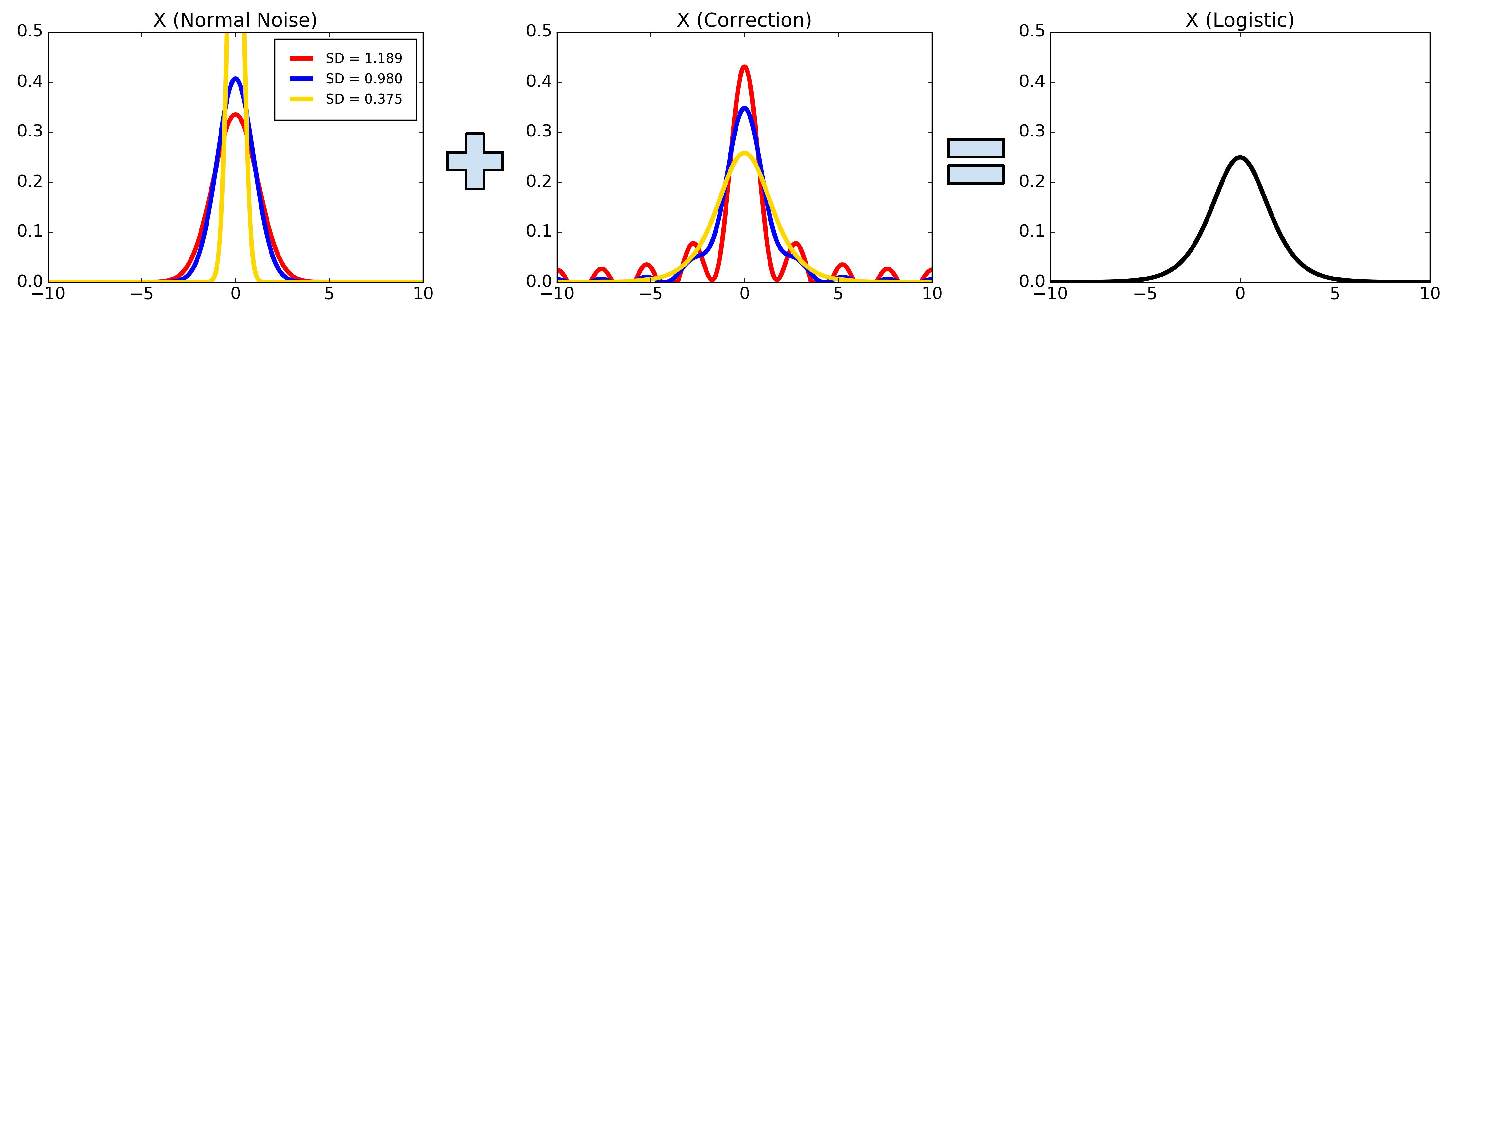
\includegraphics[width=1\textwidth]{mh_convolution_diagram_v2}
    \caption{
    Three examples of $X_{\rm norm}$ and $X_{\rm corr}$ distributions that convolve to form the
    standard logistic distribution. We use three standard deviation values of $X_{\rm norm}$. The
    two red curves convolve to form the logistic, etc. The $y$-axis is capped at 0.5 for
    readability. This figure must be viewed in color.
    }
    \label{fig:deconvolution}
    %\vspace{-10pt}
\end{figure}

It is important to understand why we use Equations~\ref{eq:deconvolution} and~\ref{eq:criteria}. The
deconvolution process allows us to use $\Delta' + X_{\rm corr}$ as a proxy for $\Delta + X$. It
works because if we know the distribution\footnote{Computing the distributions of $\varepsilon$ and
$X_{\rm norm}$ reduces to finding their standard deviations.} of $\varepsilon$ (from
Equation~\ref{eq:relationship}), then we can pretend that our $\Delta'$ is in fact $\Delta$. To
``insert'' $\varepsilon$ into our test, we deconvolve $X$ so that one of its components, $X_{\rm
norm}$, plays the part of $\varepsilon$. In light of our revised MH test, the previous discussion
raises the question: in an iteration of MCMC with current $\theta$ and proposed $\theta'$, how do
we know the distribution of $X_{\rm corr}$? We need the correct distribution to sample the
\emph{values} of $X_{\rm corr}$ appropriately. This procedure consists of three major steps.

\begin{enumerate}[noitemsep]
    \item We first need to estimate the standard deviation of $X_{\rm norm}$ (i.e. the standard deviation of $\Delta'$). We use one minibatch data to complete this task. From the proof of Lemma~\ref{lem:gaussian}, we know the randomness comes from $\frac{N}{n}\sum_{i=1}^n \left(\log p(x_i|\theta') - \log p(x_i|\theta) \right)$. Thus, ${\rm var}(\Delta') = \frac{N^2}{n^2}\sum_{i=1}^n{\rm var}\left (  \log p(x_i|\theta') - \log p(x_i|\theta) \right ) = \frac{N^2}{n}{\rm var}\left (  \log p(x_i|\theta') - \log p(x_i|\theta) \right )$. We use data instances in one minibatch to estimate the ${\rm var} \left (  \log p(x_i|\theta') - \log p(x_i|\theta) \right )$. Since there are $n$ data instances in one minibatch, the estimation of ${\rm var} \left (  \log p(x_i|\theta') - \log p(x_i|\theta) \right )$ has high accuracy. In our experiments (see Section~\ref{sec:experiments}) we also use the complete data to obtain the population variance of $\left (  \log p(x_i|\theta') - \log p(x_i|\theta) \right )$, and use the nonparametric Bootstrap to estimate the ${\rm std(std}(\Delta'))$, so that we can construct the confidence interval of ${\rm std}(\Delta')$ to reveal the accuracy of our estimation.

	\item If the ${\rm std}(\Delta') > 1.2$, the decomposition of $X$ (i.e. Equation~\ref{eq:deconvolution}) is unstable. We consume more minibatches to decrease the ${\rm std}(\Delta')$. We update the value of $\Delta'$ by $\Delta' = (k\Delta'_{\rm old} + \Delta'_{\rm new}) / (k+1)$, where $\Delta'_{\rm old}$ is the existing $\Delta'$ which uses $k$ minibatches to computed (usually $k=1$), and $\Delta'_{\rm new}$ is the $\Delta'$ computed from the new minibatch. We also update the value of ${\rm std}(\Delta')$ by ${\rm std}(\Delta') = \sqrt{\left ( k^2 {\rm var}(\Delta'_{\rm old}) + {\rm var}(\Delta'_{\rm new}) \right ) / (k+1)^2}$. Thus, we can decrease the ${\rm std}(\Delta')$ by consuming more data until the ${\rm std}(\Delta') > 1.2$. With help of temperature (see Section~\ref{ssec:discussion}), we will show that usually the mean of minibatch consumed per iteration is below 2 in Section~\ref{sec:experiments}. Later our efficiency analysis in Section~\ref{sec:theory} will reveal that the number of data instance consumed by our algorithm is much fewer than that of existing algorithms.

    \item Once we have ${\rm std}(\Delta')$, we can determine the distribution of $X_{\rm corr}$
    from standard deconvolution techniques. These rely on the well-known fact that the Fourier
    transform of a convolution is the product of the individual Fourier transforms. In practice, we
    pre-compute distributions of $X_{\rm corr}$ for different ${\rm std}(\Delta')$ values to
    facilitate the sampling process.
\end{enumerate}

Algorithm~\ref{alg:our_algorithm} describes our MH test within the MCMC algorithm.

\subsection{Discussions and Practical Considerations of the New MH Test}\label{ssec:discussion}

\SetKwInOut{Input}{Input}
\SetKwInOut{Output}{Output}
\begin{algorithm}[t]
\Input{Number of samples $T$, minibatch size $m$, pre-computed $X_{\rm
corr}$ distribution, and initial sample $\theta_0$.}
\Output{A chain of $T$ samples $\{\theta_1, \ldots, \theta\}$ from $p(\theta)$\;
MAP/ML estimation.}
\For{$t=\{1, \ldots, T\}$}{
    Propose a candidate $\theta'$\ from proposal distribution\;
    Draw a minibatch of $m$ samples, compute $\Delta'(\theta',\theta)$ and ${\rm std}(\Delta')$ for this sample\;
    \While {${\rm std}(\Delta') \ge 1$} {
    	Draw $m$ more samples to augment the current minibatch, and update $\Delta'$ and ${\rm std}(\Delta')$ \;
    }
    Let $\sigma = \sqrt{1 - {\rm std}(\Delta')^2}$, draw a normal variable $X_n \in Norm(0,\sigma)$ and
    $X_c$ from the correction distribution\;
        
        \eIf{$X_c + X_n + \Delta' > 0$}{
            Accept the candidate, $\theta_{t+1} = \theta'$\;
        }{
            Reject and re-use the old sample, $\theta_{t+1} = \theta$\;
        }
    
}
\caption{A description of our MH test within the MCMC algorithm.}
\label{alg:our_algorithm}
%\vspace{-10pt}
\end{algorithm}

\textbf{The Convolution}. Figure~\ref{fig:deconvolution} demonstrates
Equation~\ref{eq:deconvolution} and provides three (color-coded) examples of densities for $X_{\rm
norm}$ and $X_{\rm corr}$. The density of $X$, a logistic random variable with mean $\mu = 0$ and
scale $s=1$, is known, as are the $X_{\rm norm}$ densities for different standard deviations. The
deconvolution provides us with the $X_{\rm corr}$ distributions. Note, however, that as the standard
deviation of $X_{\rm norm}$ increases, the $X_{\rm corr}$ distribution becomes increasingly unstable
and ``bumpier'', because the logistic curve has fatter tails than Gaussians. In addition, we cap
the standard deviation possibilities of $X_{\rm norm}$ at $\approx 1.2$ in our experiments. In our
experiments, we discretize the possible standard deviations of $X_{\rm norm}$, and we also limit the
densities to consider the range $[-10,10]$ as shown in Figure~\ref{fig:deconvolution}.

\textbf{Variance Preconditioning}. Returning to the discussion from Section~\ref{sec:introduction},
our test requires a variance check. Equation~\ref{eq:deconvolution} means that the variance of $X$,
which is $\pi^2/3\approx 3.29$ is an upper bound on the variances of $X_{\rm norm}$. Therefore, the
test cannot work if the variance of $X_{\rm norm}$ is too large. The standard deviation of $X$
is about $\sqrt{3.29}\approx 1.81$, so this bounds ${\rm std}(X_{\rm norm})$ (as well as ${\rm
std}(\Delta')$). From the discussion above, we bound the standard deviation at 1.2 so that $X_{\rm
corr}$ can handle the remaining noise. Recall from Section~\ref{ssec:deltas_minibatch} that we
estimate the ${\rm std}(X_{\rm norm})$ each iteration. If the variance/standard deviation test
fails, then we can (a) skip the iteration, (b) increase the minibatch size, (c) change the proposal
to decrease step sizes, or (d) increase temperature, as we now discuss.

\textbf{Temperature}. One way to satisfy the variance precondition is to increase the temperature of
the target distribution. For a temperature $T>1$, the augmented target distribution would become
\begin{equation}\label{eq:log_temperature}
\log p(\theta \mid x_1,\ldots,x_N) \approx \log p(\theta) + \frac{1}{T}\frac{N}{n} \sum_{i=1}^n\log p(x_i \mid \theta).
\end{equation}
with an extra $1/T$ term augmented. As the temperature increases, the values of $\Delta'$ get
smaller in absolute value, thus reducing variance. The flatter posterior results in easier mixing.




\section{Analysis}\label{sec:theory}

In this section, we first perform an error analysis for our new
acceptance test. Second, we follow the implications of this analysis for accuracy of
the estimated target distribution. Third, we compare the speed and accuracy of
our test with prior work. Due to space constraints, all our proofs
are in Appendix~\ref{app:proofs}.

We first introduce some notation. Let our true (full dataset) and
approximate (minibatch) acceptance probabilities be $P_a = g(\Delta) =
\Pr(\Delta + X > 0)$ and $P_a' = \Pr(\Delta' + X_{\rm corr} > 0)$.
Define $X_{\xi} = \varepsilon - X_{\rm norm}$ which means, invoking
Equations~\ref{eq:relationship} and~\ref{eq:deconvolution}, that
$X_\xi$ is the random variable characterizing the accuracy of our
$X_{\rm norm}$.  Thus, $\Delta' = \Delta + X_{\rm norm} + X_\xi$. We
assume the standard deviation of $X_{\rm norm}$ is less than
$\pi/\sqrt{3}$, so that we can use Equation~\ref{eq:deconvolution}.
We denote $F_X(x)$ as the CDF of $X$.

We use some terms from standard Markov chain theory~\cite{Meyn2009}. Let the \emph{transition
kernels} of MCMC on complete and minibatch data at step $i$ be $P_i$ and $P_i'$, respectively. When
these kernels (e.g., $P_i$) are applied on a probability distribution $D_1$, they generate a new
distribution $D_2$, which we write as $P_i \circ D_1 = D_2$. Define $\pi$ to be the stationary
distribution obtained by $P_i$, and $\pi_i'$ to be the stationary distribution obtained by $P_i'$
($\pi'$ needs a subscript in this case).  Finally, we indicate the \emph{total variation distance}
between two kernels using $\| \cdot \|$.

Our first result shows that the distance $\|P_i\circ D - P_i'\circ D\| \le 4\zeta \ell$ for all
distributions $D$.

% Our first result shows that the distance between $P_i$ and $P_i'$ is proportional to our estimation
% error $X_{\xi}$.

\begin{lemma}\label{lem:theory1}
If $|X_\xi| < \zeta$ and $|\nabla F_X(x)| < \ell$ for all $x$, then $\|P_i\circ D-P_i'\circ D\| \le
4\zeta \ell \;\;\forall D$.
\end{lemma}

%% \begin{proof}
%% See Appendix~\ref{app:theory1}.
%% \end{proof}

Thus, the accuracy of our transition kernel $P_i'$ is related to the quality of our estimated
$X_{\rm norm}$. We next show that ${\rm Var}(\Delta')$ is roughly proportional to the step size of
our proposer.

\begin{lemma}\label{lem:theory2}
For one step sampling from $\theta$ to $\theta'$, if the jumping step $\|\theta - \theta'\|_2 <
\epsilon$, and the gradient of the log likelihood is bounded by a constant factor, i.e. $\|\nabla
(\log \Pr(x_i\mid \theta))\|_2 < k$, the variance of $\Delta'$ is bounded by $4\epsilon^2 k^2
(m-\frac{m(m-1)}{N-1})$, where $m$ is the minibatch size, and $N$ is the total data size.
\end{lemma}

%% \begin{proof}
%% See Appendix~\ref{app:theory2}.
%% \end{proof}

Since ${\rm Var}(\Delta') < 4\epsilon^2 k^2 (m - \frac{m(m-1)}{N-1}) $, we can assume the maximum
value of $X_{\xi}$ is proportional to the standard deviation of $\Delta'$, i.e. $\epsilon$. Thus, we
can assume $\zeta=\epsilon C$, where $C$ is a constant factor. We finally introduce
Theorem~\ref{thm:theory3} to characterize the convergence of our samples.

\begin{theorem}\label{thm:theory3}
Assume $\pi$ satisfies $\|P_i \circ D_0 - \pi\| \leq \eta \|D_0 - \pi\|$, where $\eta \in [0, 1)$ for
all distributions $D_0$. Also assume there exists $0 < \rho_t < 1$ such that $\|P'_i \circ D -
\pi_i'\| \leq 2\rho_i \;\; \forall D$. We can get $\| P_t' \circ P_{t-1}' \circ \cdots \circ P_1' \circ D_0 - \pi
\| \leq \sum_{s=1}^t \{\prod _{u=s+1}^t \rho_u (1-\alpha_u)\} \rho_s \alpha_s + \alpha_t $, where
$\alpha_i = \frac{\epsilon_i C }{1-\eta}$ and $\epsilon_i$ is the step size at iteration $i$.
\end{theorem}

%% \begin{proof}
%% See Appendix~\ref{app:theory3}.
%% \end{proof}

Theorem~\ref{thm:theory3} indicates that the difference between the target and sampled distributions
consists of two components: $\rho_i$, which is determined by the efficiency of $P'_i$, and the
$\alpha_i$s, which are determined by the error of our transition kernels. These involve competing
objectives: the larger the step size, the more efficient the $P_i'$ but its error increases.  The
reverse happens with a step size too small.

We explore the efficiency of our minibatch MH test. Theorem~\ref{thm:efficiency} indicates that our minibatch MH test only requires a constant number of instances for each step, however, recall the Lemma~\ref{lem:efficienty_cutting}, the adaptive minibatch MH test requires $O(\sqrt{N})$ number of data instance for each step. Thus, We show that our proposed minibatch MH test is much higher efficient than the known minibatch algorithms. 

\begin{theorem}\label{thm:efficiency}
We require $\frac{ C^2 \rho^2 }{\sigma^6 \varepsilon^2}$ minibatch size to ensure $|P_a -P_a'| < \varepsilon$, where $C$ is a positive constant which is smaller than 0.4748, $\sigma^2 $ and $\rho$ is the second and third moment of $(\nabla\log \Pr(x_i|\theta) - \nabla\log\Pr(x_i|\theta')) - E\left[ \nabla\log \Pr(x_i|\theta) - \nabla\log\Pr(x_i|\theta')\right]$, $P_a$ is the accept rate from the complete data, $P_a'$ is the accept rate from minibatch data by our algorithm, $\theta$ is the current parameter, and $\theta'$ is the proposed parameter. 

\end{theorem}


\section{Experiments}\label{sec:experiments}

We conduct three sets of experiments to explore the benefits of our minibatch MH test and to
benchmark it with previous work. In Section~\ref{ssec:gaussians}, we show that our test enables
samples to converge to the posterior distribution of a heated Gaussian mixture model. In
Section~\ref{ssec:logistic}, we analyze its efficiency on logistic regression. In
Section~\ref{ssec:nets}, we apply the test for deep learning.
Appendices~\ref{app:gaussian},~\ref{app:logistic}, and~\ref{app:nnet} contain more detailed
information on these respective experiments.

\subsection{Mixture of Gaussians}\label{ssec:gaussians}

We start with a simple Gaussian mixture model, borrowing an experiment from~\cite{langevin_2011}.
The parameter is 2-D, $\theta = (\theta_1,\theta_2)$, and the parameter/data generation process is
\begin{equation}\label{eq:data_generation}
(\theta_1,\theta_2) \sim \mathcal{N}((0,0), {\rm diag}(\sigma_1^2, \sigma_2^2));\quad \quad x_i \sim
0.5 \cdot \mathcal{N}(\theta_1, \sigma_x^2) + 0.5 \cdot \mathcal{N}(\theta_1+\theta_2, \sigma_x^2).
\end{equation}
We set $\sigma_1^2 = 10, \sigma_2^2 = 1$ and $\sigma_x^2=2$. Fixing $\theta = (0,1)$, we draw 10000
data points so that the target distribution is $p(\theta)\prod_{i=1}^{10000}p(x_i\mid \theta)$, with
the prior based on the $\theta$ generation process in Equation~\ref{eq:data_generation}. This
results in rather sharp posterior modes and high ${\rm std}(\Delta')$ estimates, so we apply a
temperature $T=110$ to reduce ${\rm std}(\Delta')$. Taking logs, we get the target as shown in the
far left of Figure~\ref{fig:gauss_mix_1}.

We run MCMC with our MH test using minibatch size $m=200$. We also run this using standard
full-batch MCMC (``standard sampling'') with the standard test from Equation~\ref{eq:traditional}, and the method
from~\cite{cutting_mh_2014} (``adaptive sampling''). For the latter, we also use $m=200$ and
increment minibatches by that amount within an iteration if necessary. The tolerance for making a
decision is $\epsilon=0.1$. To make comparisons easier, all three use the same random walk proposer
with covariance $\Sigma={\rm diag}(0.03, 0.03)$. This is a poor proposer, but it is sufficient for
our purposes as the quality of the samples will be primarily due to the MH test. All methods are run
10000 times to collect 10000 samples.

\begin{figure}[t]
    \centering
    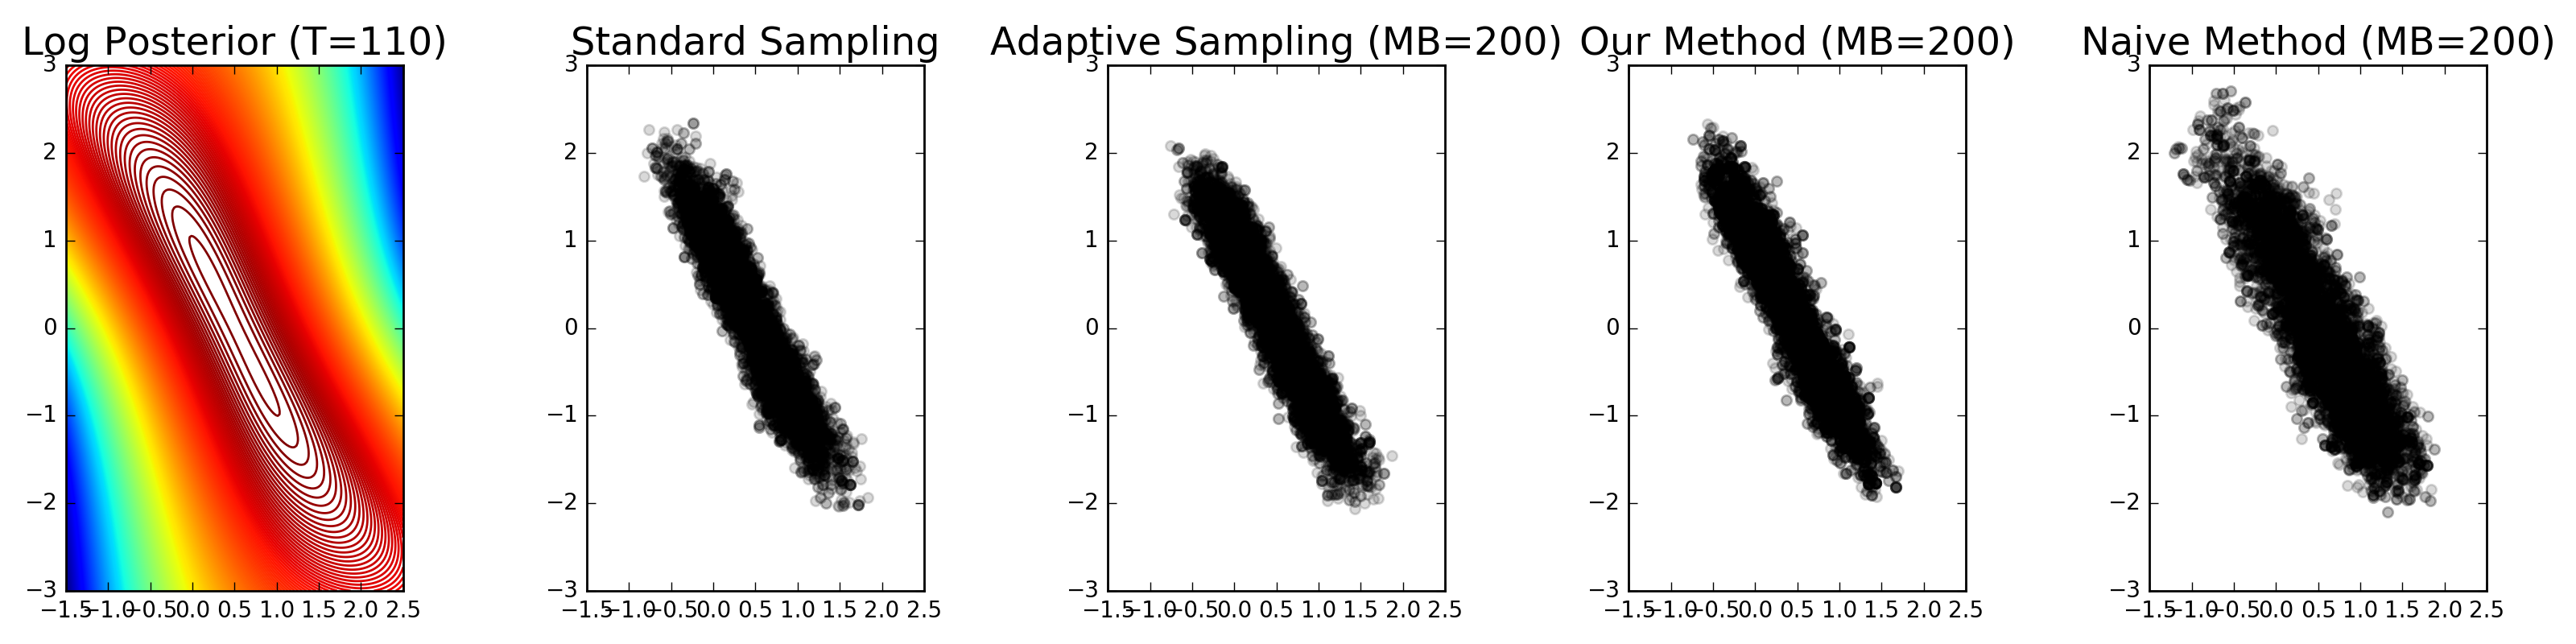
\includegraphics[width=1\linewidth]{cloud_v01.png}
    \caption{
    The log posterior contours (temperature 110) and three scatter plots of sampled $\theta$ values.
    }
    \label{fig:gauss_mix_1}
    %\vspace{-10pt}
\end{figure}

\begin{figure}[t]
    \centering
    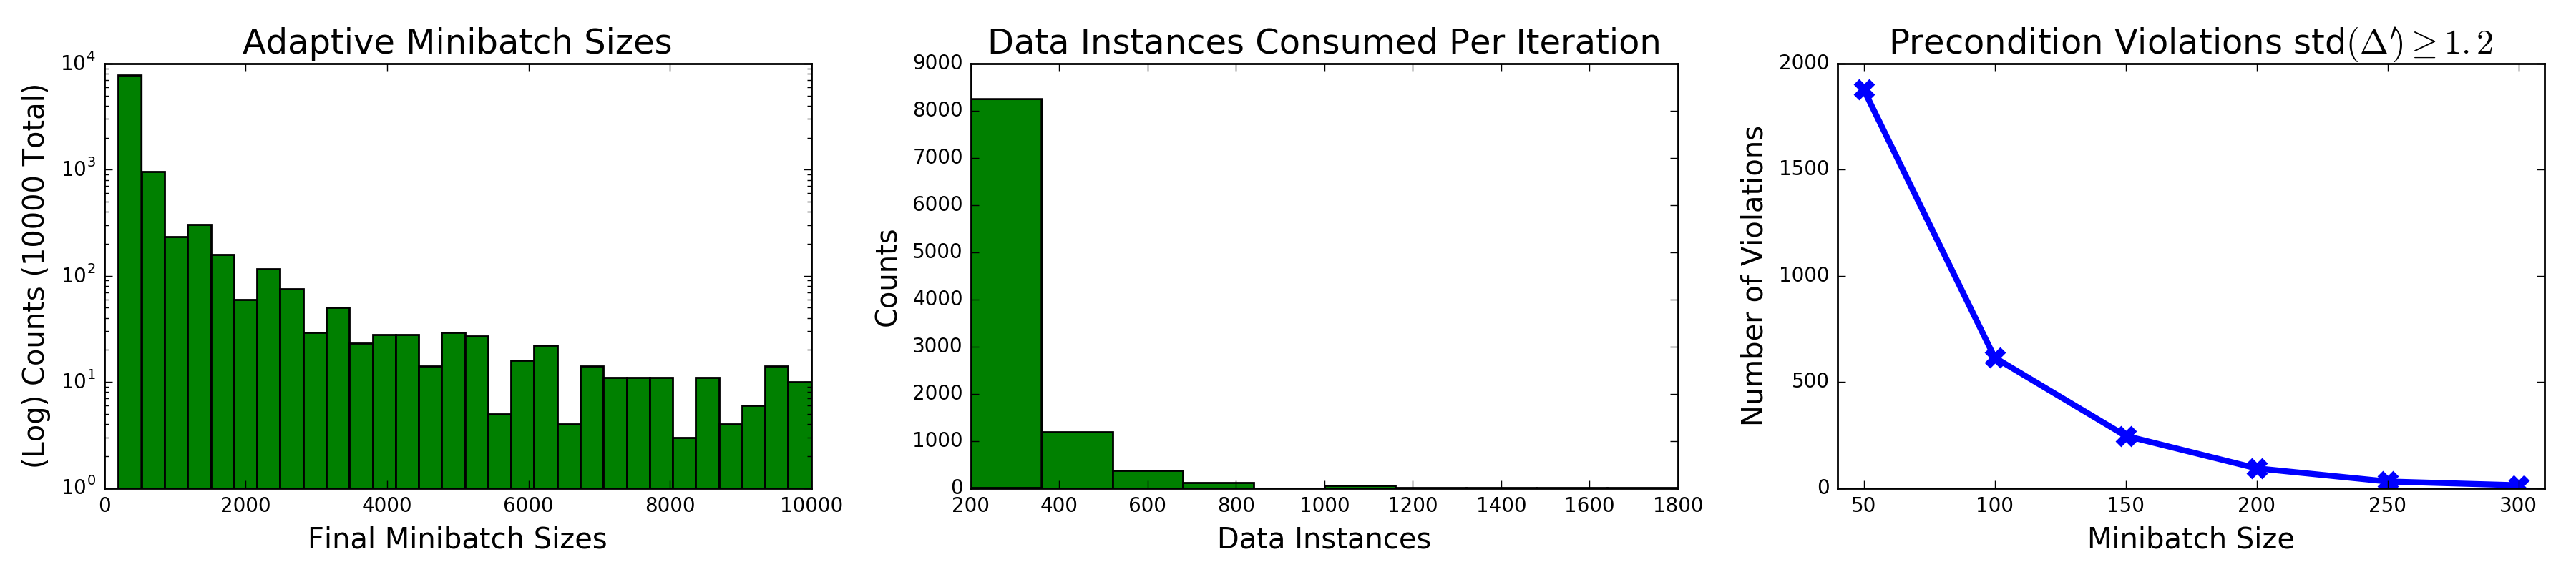
\includegraphics[width=1\linewidth]{adaptive_and_ours_information_v01.png}
    \caption{
    Histograms of minibatch sizes and ${\rm std}(\Delta')$ values, along with ``${\rm std}(\Delta')$
    violations'' (right).
    }
    \label{fig:gauss_mix_2}
    %\vspace{-10pt}
\end{figure}

\begin{figure}[t]
    \centering
    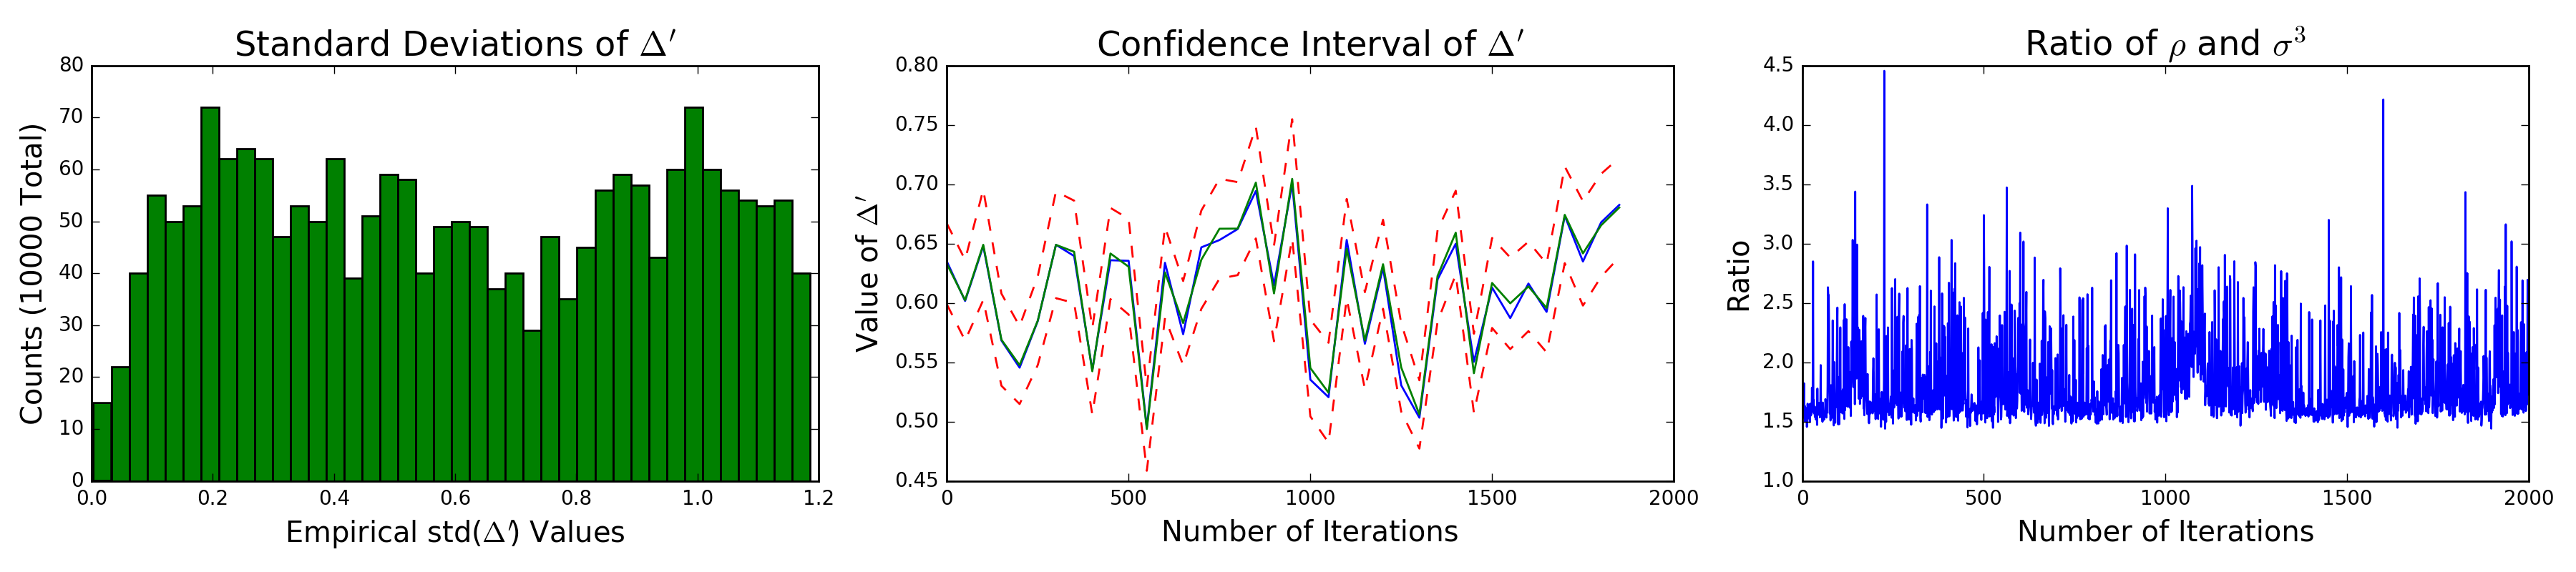
\includegraphics[width=1\linewidth]{CI_v01.png}
    \caption{
    Histograms of ${\rm std}(\Delta')$, confidence interval of ${\rm std}(\Delta')$ (middle), along with $\rho / \sigma^3$ (right).
    }
    \label{fig:gauss_mix_3}
    %\vspace{-10pt}
\end{figure}

Figure~\ref{fig:gauss_mix_1} shows scatter plots of the resulting $\theta$ samples for the four
methods, with darker regions indicating a greater density of points. The first three methods obtain the
same rough form of the posterior, so our MH test can indeed result in the same posterior as the
other two methods. However, the fourth method (i.e. just treat the $\Delta'$ which comes from minibatch as $\Delta$ which comes from the complete data) reveals wider spread distribution than the posterior. From Figure~\ref{fig:gauss_mix_1} we illustrate our proposed method can obtain the samples which have almost the same distribution as the standard MH test from the complete data, adaptive minibatch test, and the true posterior. Meanwhile, we show the benefits of our minibatch method compared with the naive minibatch method.  

Figure~\ref{fig:gauss_mix_2} (to the left) shows a histogram of the final minibatch sizes used by
the adaptive subsampling method each iteration (on a log scale for readability).  Usually, the method
can make a decision with 200 samples. Occasionally, however, it must use all 10000 points, resulting
in lots of wasted computation.  For this particular experiment, that happened eight times. The mean of adaptive minibatch size is 520 which is roughly close to $\sqrt{N}$ (i.e. 100). This number validates the claims of Theorem~\ref{thm:efficiency}. In
contrast, our method keeps the minibatch size around 200. Figure~\ref{fig:gauss_mix_2} (in the middle) shows a histogram of the minibatch size, and the mean of our minibatch size is 247. 
The third plot in Figure~\ref{fig:gauss_mix_2} investigates the number of times ${\rm std}(\Delta')
\ge 1.2$ for only consuming one minibatch data. For six minibatch sizes (50, 100, 150, 200, 250, and 300), we ran MCMC with
our MH test five times and averaged the number of ``violations.'' As the size increases, the
number of violations decreases, as expected.

Figure~\ref{fig:gauss_mix_3} (to the left) shows a histogram of ${\rm std}(\Delta')$. Figure~\ref{fig:gauss_mix_3} (to the middle) shows the confidence interval of our estimated ${\rm std}(\Delta')$ at each iteration \footnote{In order to show the confidence interval clearly, we use moving smooth to smooth the confidence interval, and plot each value by interval of 50 iterations}. The blue line represents the standard deviation comes from the complete data, which can be treated as the ``true'' ${\rm std}(\Delta')$, the green line represents our estimation of ${\rm std}(\Delta')$ from the minibatch, and the two red dash lines represent the confidence interval of ${\rm std}(\Delta')$ by adding / subtracting one ${\rm std(std(}\Delta'))$. This figure indicates that our estimation of ${\rm std}(\Delta')$ from one minibatch data is accurate. Figure~\ref{fig:gauss_mix_3} (to the right) shows the value of $\rho/\sigma^3$ at each iteration. Recall Theorem~\ref{thm:efficiency}, the number of data instance required is $\frac{4 \ell^2 C^2 \rho^2 }{\sigma^6 \varepsilon^2}$. This figure reveals that $\rho/\sigma^3$ is roughly a constant, which means the data required for each iteration is a constant value which has nothing to do with the $N$.


\subsection{Logistic Regression}\label{ssec:logistic}

We next use logistic regression for the binary classification of 1s versus 7s in the MNIST
dataset~\cite{lecun-mnisthandwrittendigit-2010}. The data has 12007 and 1000 training and testing
points, respectively (we used a random subset of the test data). The proposer is again a random walk
with covariance matrix $0.1I$ for the $784\times 784$ identity matrix $I$. We set the posterior
temperature at $T=3000$. We set the minibatch size $m=50$ and compare with adaptive sampling with
tolerance 0.02.

Figure~\ref{fig:logistic_fig} shows the prediction accuracy and log likelihood on the test set as a
function of the cumulative training data points processed. Our test increments the cumulative data
by a fixed amount per iteration, but the adaptive method may require more data per iteration.  We
see that our minibatch MH test is more efficient; it has similar or better performance while
consuming fewer data points.

\begin{figure}[t]
    \centering
    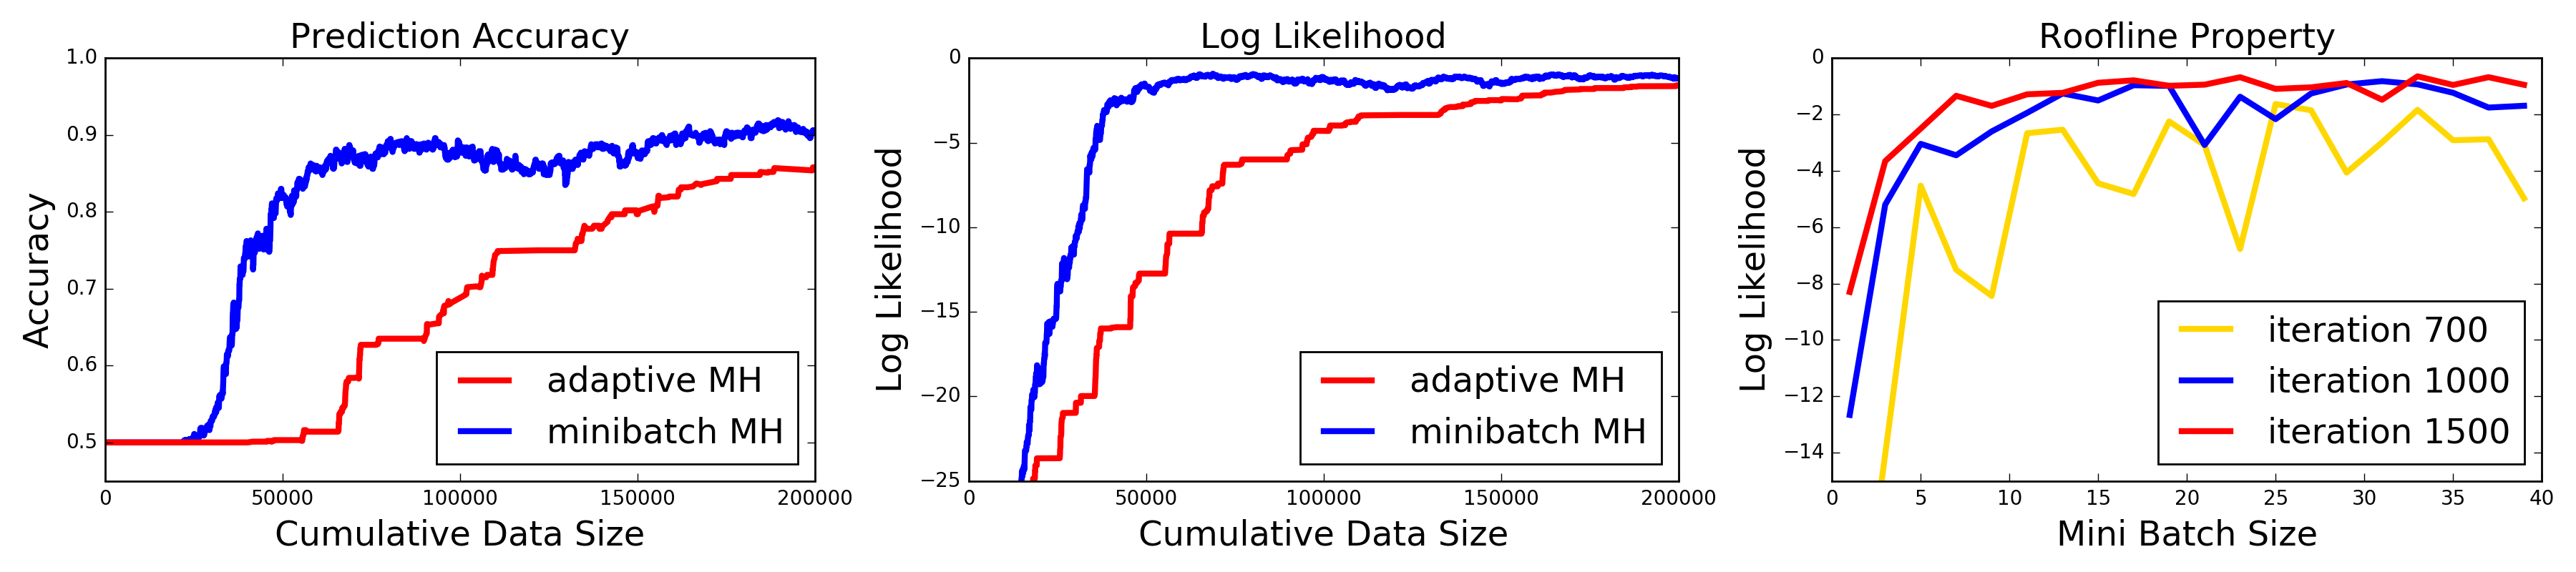
\includegraphics[width=1\linewidth]{exp2.png}
    \caption{Logistic regression performance (accuracy/log likelihood) and minibatch size analysis.}
    \label{fig:logistic_fig}
    \vspace{-10pt}
\end{figure}

\begin{figure}[t]
    \centering
    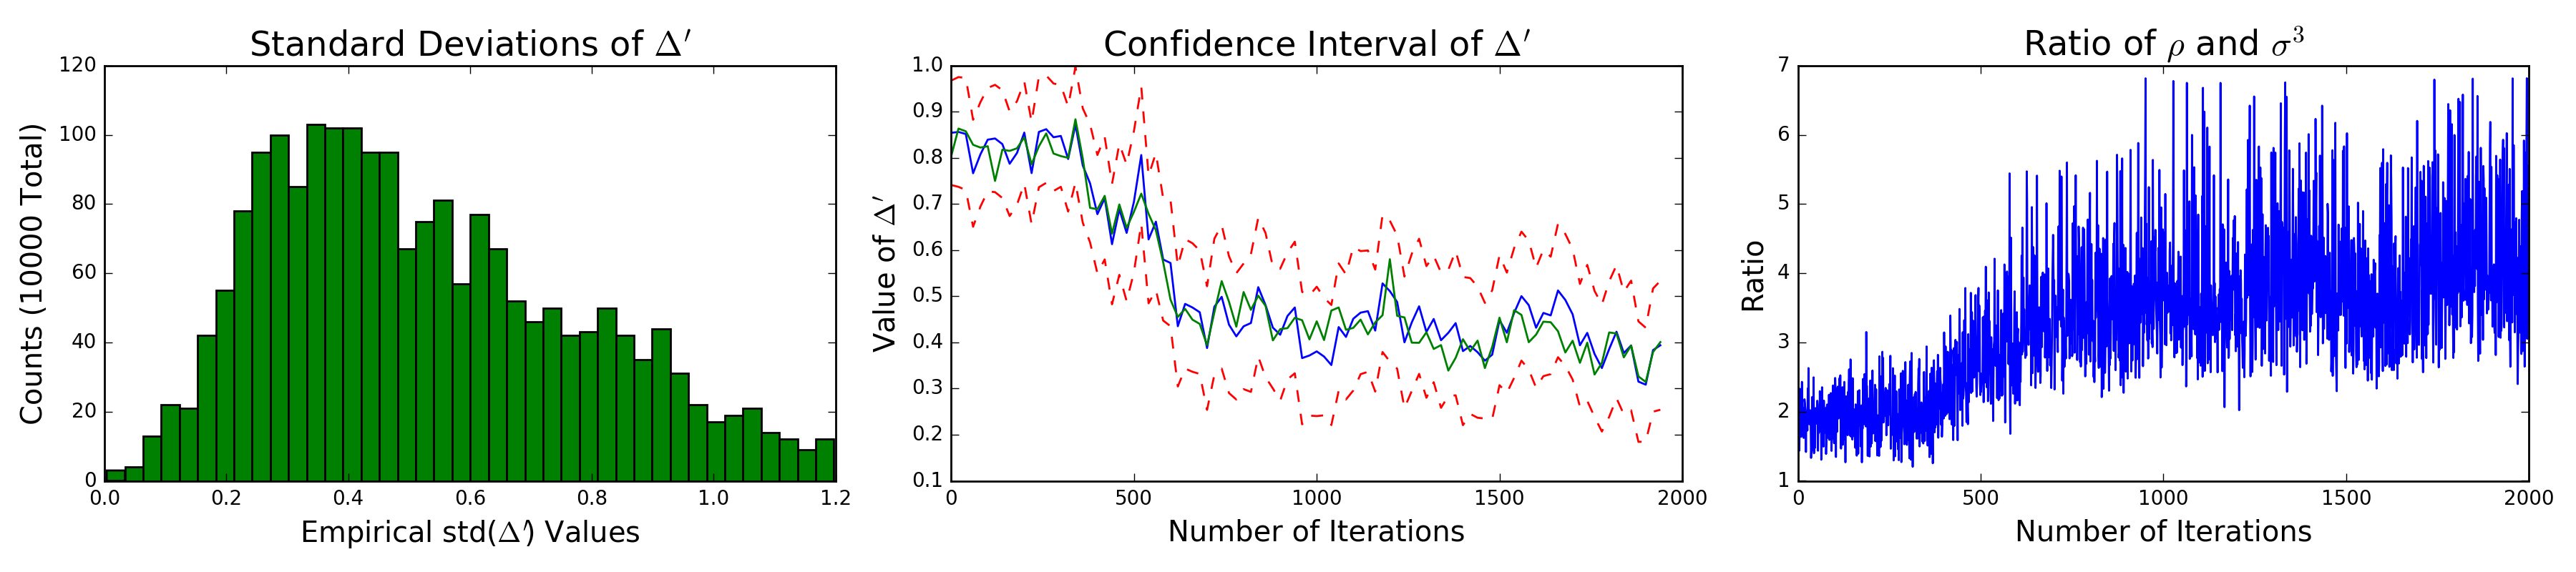
\includegraphics[width=1\linewidth]{CI_v02.png}
    \caption{
    Histograms of ${\rm std}(\Delta')$, confidence interval of ${\rm std}(\Delta')$ (middle), along with $\rho / \sigma^3$ (right).
    }
    \label{fig:exp_3}
    %\vspace{-10pt}
\end{figure}

The third plot of Figure~\ref{fig:logistic_fig} shows performance based on minibatch size. The
parameter is evaluated on the test set after training iterations 700, 1000, and 1500. For those
three cases, when the minibatch size increases beyond about 10, the performance of the sampled data
will not improve with a large minibatch size. This makes sense because the error of our MH test is
proportional to our estimation error of ${\rm std}(\Delta')$, and as the minibatch increases, ${\rm
std}(\Delta')$ decreases. Beyond a certain standard deviation (or minibatch) threshold, the error in
our minibatch MH test is negligible.

Similar as the Subsection~\ref{ssec:gaussians}, we use Figure~\ref{fig:exp_3} to reveal the accuracy of our estimation of ${\rm std}(\Delta')$ and stability of $\rho/\sigma^3$.


\subsection{Neural Network Optimization}\label{ssec:nets}

In this experiment, we apply our minibatch MH test with a Stochastic Gradient Hamiltonian
Monte Carlo (SGHMC)~\cite{sghmc_2014} proposer to sample the complete parameters for a fully
connected neural network. We use the Higgs data set from the UCI dataset~\cite{Lichman:2013}, which
is a binary classification task with one million instances, each of which are 28-dimensional. The
network we use has four layers: the first is the input, the last is the softmax, and the
intermediate ones apply the sigmoid activation unit.  We also employ dropout and batch
normalization~\cite{icml2015_ioffe15}.  In order to control ${\rm std}(\Delta')$, we initialize the
temperature at 1000, and adjust it at iteration $i$ according to $T_i = \max\{1,
1000/(i+1)^{0.5}\}$.

For our comparison baseline, we train the same network architecture using the Adaptive Gradient
Descent method~\cite{adapGrad}. Since the frequencies of the features are quite different, we use
the same strategy as in Adaptive Gradient to rescale the gradient before applying SGHMC. We
implement our MH test and SGHMCin the open-source BIDMach project~\cite{canny2013bidmach}.  

Figure~\ref{fig:nnet_fig} illustrates our experiment results and reveals that SGHMC with our
minibatch MH test achieves higher log likelihood than the baseline. By comparing SGHMC with and
without our minibatch MH test, we see that our MH test has limited benefit. Because we decrease the
step size quickly, the acceptance rate of SGHMC is already high, so there is little need to test.
% Daniel's note: Haoyu said he cannot increase the step size without it violating the variance
% condition.

\begin{figure}[t]
    \centering
    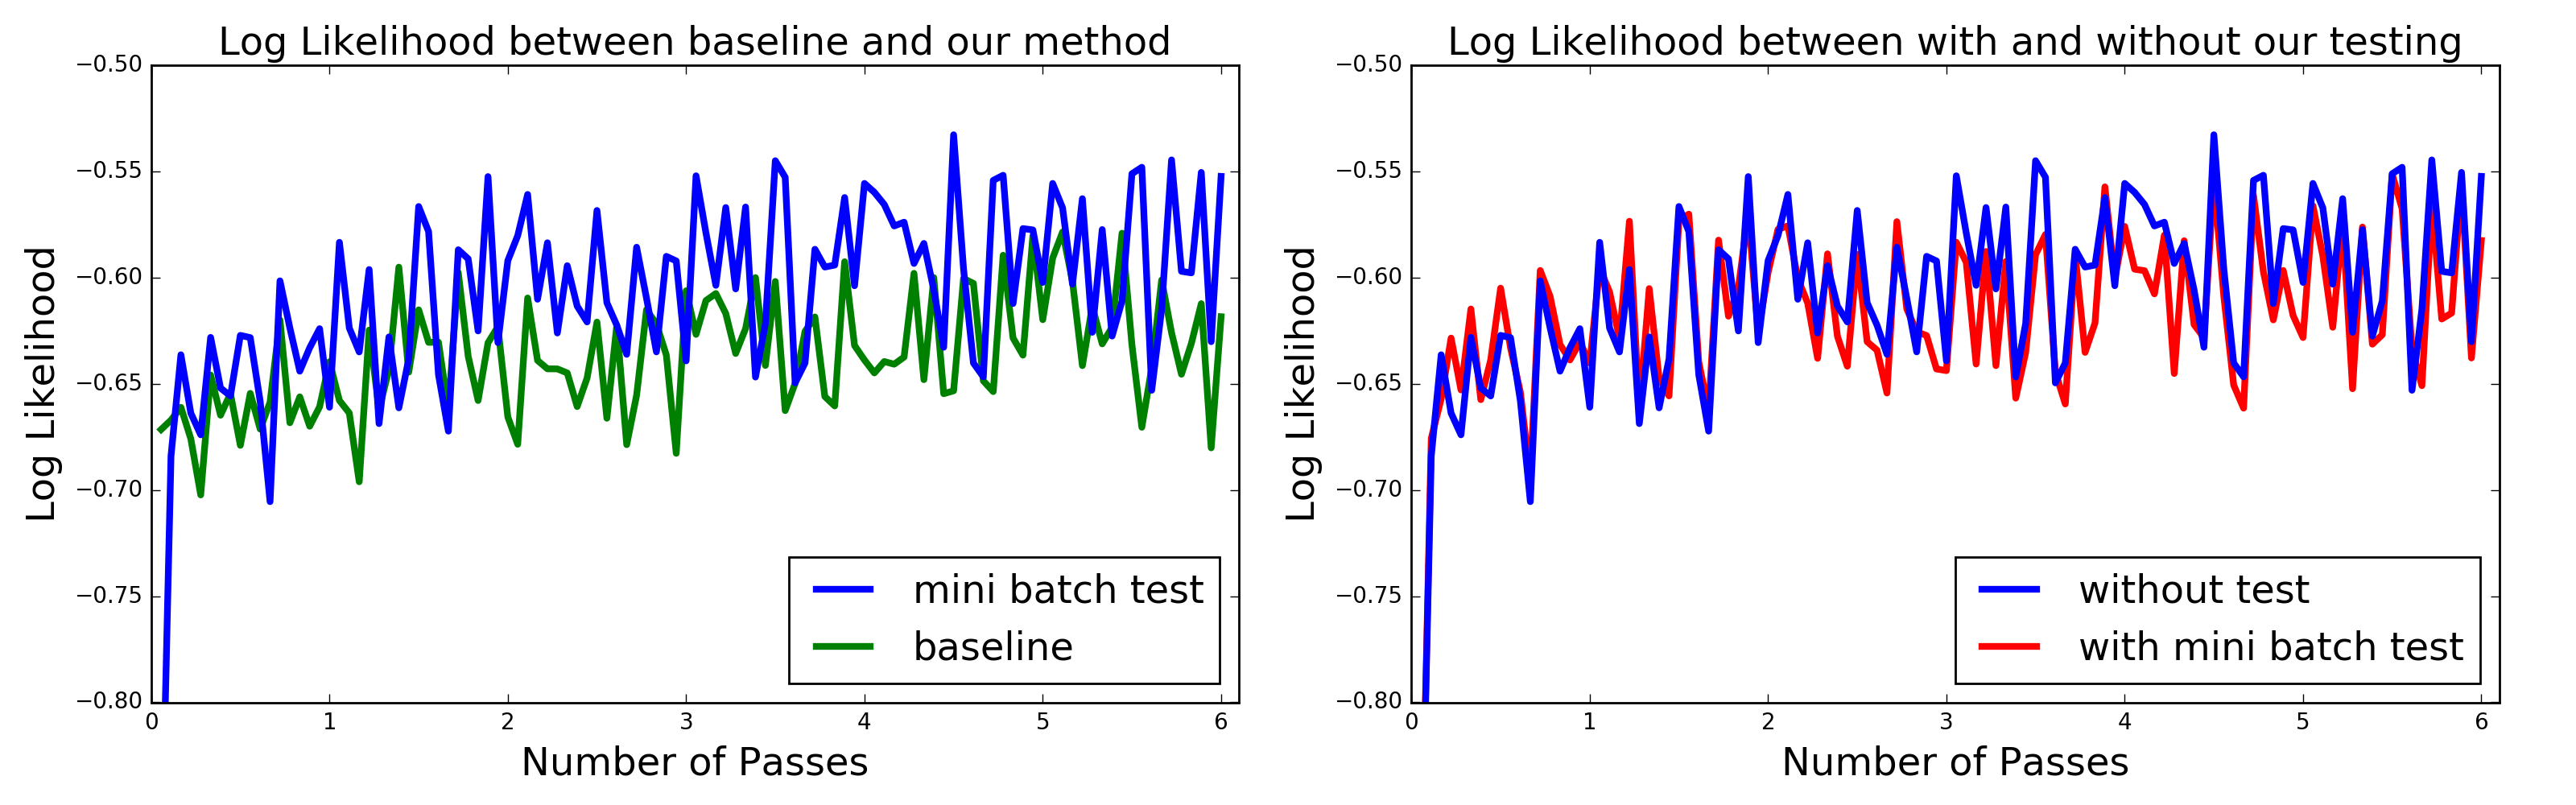
\includegraphics[width=1\linewidth]{exp3}
    \caption{Log likelihood versus number of passes for optimization of neural network.}
    \label{fig:nnet_fig}
    \vspace{-10pt}
\end{figure}




\section{Conclusions}\label{sec:conclusion}

In this paper, we have derived a new MH test for minibatch MCMC methods. We demonstrated how a
simple deconvolution process allows us to use a minibatch approximation to the full data tests. We
experimentally show the benefits of our test on Gaussian mixtures, logistic regression, and deep
learning.  Straightforward directions for future work include running more experiments with a
particular focus on investigation of the variance precondition.  More elaborate extensions include
combining our results with Hamiltonian Monte Carlo methods, providing a recipe for how to use our
algorithm (following the framework of~\cite{sgmcmc_2015}), or integrating parallel
MCMC~\cite{conf/uai/AngelinoKWSA14,conf/icml/AhnSW14} concepts.


\small
\bibliography{nips_2016}
\bibliographystyle{ieeetr}
\normalsize

\clearpage
\appendix

\begin{center}
{\Large Outline of Appendix}
\end{center}

In this appendix, we describe the following topics, with an emphasis on clarity and understanding:

\begin{itemize}[noitemsep]
    \item Proofs for material in Section~\ref{sec:theory}.
    \item More information on Section~\ref{ssec:gaussians}.
    \item More information on Section~\ref{ssec:logistic}.
    \item More information on Section~\ref{ssec:nets}.
\end{itemize}

\section{Proofs}\label{app:proofs}

\subsection{Proof of Lemma~\ref{lem:efficienty_cutting}}\label{app:lem_efficiency}

If the minibatch size is $n$, we first compute the probability that more than $n$ data instances are required for adaptive sampling method for one iteration. We denote this probability $P_{rej}$.
\[P_{rej} = \Pr \left ( 1-\phi_{n-1} \left( \frac{|\bar{l} - \frac{1}{N} \log (u\frac{p(\theta)q(\theta'|\theta)}{p(\theta')q(\theta|\theta')})|}{s} \right )  \geq \varepsilon \right ) \] 

where $s = \frac{s_l}{\sqrt{n}}\sqrt{1-\frac{n-1}{N-1}}$. \\
We define random variable $Z = \frac{1}{N}\log (uQ)$, where $Q=\frac{p(\theta)q(\theta'|\theta)}{p(\theta')q(\theta|\theta')}$. Then $Z$ has probability density function $f_Z(z) = N \exp(zN), z \in (-\infty, \frac{1}{N} \log Q]$.

\begin{align*} 
P_{rej}&=  \Pr \left( 1-\varepsilon \geq \phi_{n-1} \left( \frac{|\bar{l} - Z|}{s_l \sqrt{\frac{N-n}{N-1}}} \sqrt{n} \right) \right) \\ 
&=  \Pr \left(\phi^{-1}_{n-1} \left (1-\varepsilon \right) \frac{s_l }{\sqrt{n}} \sqrt{\frac{N-n}{N-1}} \geq |\bar{l} -Z| \right) = \Pr \left( |\bar{l} - Z| \leq \frac{\eta s_l}{\sqrt{n}}\sqrt{\frac{N-n}{N-1}} \right) \\
&= \Pr \left(Z - \frac{\eta s_l}{\sqrt{n}}\sqrt{\frac{N-n}{N-1}} \leq \bar{l} \leq Z + \frac{\eta s_l}{\sqrt{n}}\sqrt{\frac{N-n}{N-1}} \right) \\
&= \int_{-\infty} ^{\frac{\log Q}{N}} N \exp (zN)dz \int_{z - \frac{\eta s_l}{\sqrt{n}}\sqrt{\frac{N-n}{N-1}}} ^{z+ \frac{\eta s_l}{\sqrt{n}}\sqrt{\frac{N-n}{N-1}}} \frac{1}{2L} d\bar{l} = \frac{\eta s_l}{L\sqrt{n}}\sqrt{\frac{N-n}{N-1}} \int_{-\infty} ^{\frac{\log Q}{N}} N \exp(zN) dz \\
&= \frac{\eta s_l}{L\sqrt{n}}\sqrt{\frac{N-n}{N-1}} Q
\end{align*}
 If we define the random variable $X$ the number of instance for one minibatch, we have $\Pr (X>n) = P_{rej} = \frac{\eta s_l}{L\sqrt{n}}\sqrt{\frac{N-n}{N-1}} Q, \mbox{ for } n \in [1,N], n \in Z^+$. Since $X$ is nonnegative, we have $E(X) \geq \Pr (X >x)x, \forall x$. If we choose $x=N/2$, we have $E(X) \geq \frac{\eta s_l}{L\sqrt{N/2}}\sqrt{\frac{N-N/2}{N-1}} Q \frac{N}{2} \geq \frac{\eta s_{l}Q}{2L}\sqrt{N}$.

\subsection{Proof of Lemma~\ref{lem:theory1}}\label{app:theory1}

We first prove that the difference in our acceptance rates is bounded: $|P_a - P_a'| \leq 2\zeta
\ell$ for some small constant $\zeta > 0$. Given $X_\xi = \xi$ the distance $|P_a - P_a'|$ is:
\begin{align*}
|P_a - P_a'| &= |\Pr(\Delta + X >0) - \Pr(\Delta' + X_{\rm corr} > 0)|\\
& = | \Pr (\Delta + X > 0) - \Pr (\Delta + X_{\rm norm} + \xi + X_{\rm corr} >0) |    \\
&= |\Pr (\Delta + X > 0) -\Pr(\Delta + X + \xi >0)| \\
&= |F_X(-\Delta)- F_X(-\Delta - \xi)| \\
&= |\nabla F(-\Delta) \xi + o(\xi^2)|\\
&\leq  |\nabla F(-\Delta) \xi| +| o(\xi^2)| \leq 2|\nabla F(-\Delta)| |\xi| \leq 2\ell \xi,
\end{align*}
where we use Taylor's Theorem ($o(\xi^2)$ represents higher-order terms that have smaller absolute
value) and the Triangle Inequality.  Since $|X_\xi| < \zeta$, $|P_a - P_a'| < 2 \zeta \ell$.

Next, we show the distance of new distributions obtained by applying $P_i$ and $P_i'$ on an
arbitrary distribution $D$ once is bounded if we use the same proposer, i.e.  $\|P_i\circ D -
P'_i\circ D\| \leq 4\zeta \ell \;\; \forall D$. We write $P_i(\theta \mid \theta') = P_a(\theta, \theta')
q(\theta'\mid \theta) + (1-P_a(\theta,\theta')) \delta_D(\theta' - \theta)$, where $\delta_D$
is the Dirac delta function. The total variation distance between two generated distributions is
\begin{align*}
\|P_i\circ D - P'_i\circ D\| &= \int_{\theta'} \left| \int_{\theta}((P_a-P_a') q(\theta'|\theta) + (1-P_a - 1+P_a') \delta_D(\theta -\theta')) dD(\theta) \right| d\theta' \\
&= \int_{\theta'} \left| \int_{\theta} (P_a- P_a')(q(\theta'|\theta) - \delta_D(\theta - \theta')) dD(\theta) \right|  d\theta'\\ 
&\leq 2 \zeta \ell \int_{\theta'} \left| \int_{\theta}(q(\theta'|\theta) + \delta_D(\theta - \theta')) dD(\theta) \right| d\theta'\\
&\leq 2 \zeta \ell \int_{\theta'} ( D'(\theta') + D(\theta') ) d\theta'\\
&= 4 \zeta \ell,
\end{align*}
where $D'$ is the distribution generated if we always accept the proposed point. (In the last line,
we integrate two probability density functions, resulting in a value of two.) This matches our
desired bound.

\subsection{Proof of Lemma~\ref{lem:theory2}}\label{app:theory2}

From Lemma~\ref{lem:gaussian}, only the $\sum_{i=1}^n (\log p(x_i\mid \theta') - \log p(x_i\mid
\theta))$ term brings randomness into $\Delta'$. To simplify the subsequent notation, we define
$g_i(\theta) = \log p(x_i\mid \theta)$, and $q_i = g_i(\theta') - g_i(\theta)$. Then by Taylor's Theorem:
\[
|q| = |g(\theta') - g(\theta)| = |\nabla g(\theta)^T(\theta' - \theta) + o(\theta' - \theta)^2| \leq 2\epsilon k.
\]
Thus, given $\theta$ and $\theta'$, the variance of $\Delta'$ can be written as:
\begin{align*}
{\rm Var}(\Delta') &= {\rm Var}\left[\sum_{i=1}^m g_i(\theta') - g_i(\theta)\right] = {\rm Var}\left(\sum_{i=1}^m q_i\right) \\
&= m {\rm Var} (q_i) + m(m-1) {\rm Cov}_{i \neq j}(q_i,q_j) \\
&= m{\rm Var}(q_i) - \frac{m(m-1)}{N-1} {\rm Var}(q_i) \\
&\leq 4\left(m - \frac{m(m-1)}{N-1}\right)k^2 \epsilon^2,
\end{align*}
as desired.

\subsection{Proof of Theorem~\ref{thm:theory3}}\label{app:theory3}

First, by Theorem 1 in~\cite{cutting_mh_2014}, $\|P_i \circ D_0 - \pi\| \leq \eta \|D_0
- \pi\|$ and $\|P_i\circ D-P'_i\circ D\| \leq \epsilon_i C$ for all $D$. The norm between the
stationary distributions is $\|\pi - \pi_i'\|\leq \frac{\epsilon_i C}{1-\eta}$.

Second, by Theorem 3.6 in~\cite{yang2013sequential}, we have 
\[
\| P_t' \circ \cdots \circ P_1' \circ D_0 - \pi_t \| \leq \sum_{s=1}^t \left\{\prod _{u=s+1}^t
\rho_u (1-\alpha_u)\right\} \rho_s \alpha_s,
\]
where $\alpha = \frac{\epsilon_i C}{1-\eta}$.  Thus, we get:
\begin{align*}
 \| P_t' \circ \cdots \circ P_1' \circ D_0 - \pi_0 \| &\leq \|P_t' \circ \cdots \circ P_1' \circ D_0 - \pi_t\| + \|\pi_t - \pi_0\| \\
 &\leq \sum_{s=1}^t \left\{\prod _{u=s+1}^t \rho_u (1-\alpha_u)\right\} \rho_s \alpha_s + \alpha_t,
\end{align*}
as desired.

\subsection{Proof of Theorem~\ref{thm:efficiency}}\label{app:theory4}
Since only the $\frac{N}{nT}\sum_{i=1}^n \left(\log p(x_i|\theta') - \log p(x_i|\theta) \right)$ term brings randomness into $\Delta'$. Define $X_i = \frac{N}{T}\left(\log p(x_i|\theta') - \log p (x_i|theta_t) \right)$, $\tilde{X_i} = X_i - E(X_i)$, and $Y_n = \frac{\sum_{i=1}^n \tilde{X_i}}{n}$ (i.e. $Y_n$ is the $\Delta' - E(\Delta')$). From Berry-Esseen theorem, $|F_n(x) - \Phi(x)| \leq \frac{C\rho}{\sigma^3\sqrt{n}}$, where $\Phi()$ is the CDF of standard normal distribution, $F_n()$ is the CDF of $Y_n$, $C$ is the constant parameter which is below 0.4748, $\rho = E(|\tilde{X_i}|^3)$, and $\sigma^2 = E(\tilde{X_i}^2)$. Since $\Delta'$ is an unbiased estimator of $\Delta$, the CDFs between $\Delta'$ and $\Delta + X_{\rm norm}$ has the same max gap (i.e. $\frac{C\rho}{\sigma^3\sqrt{n}}$).

From Equation~\ref{eq:criteria}, we show we want to use $\Delta' + X_{\rm corr}$ to approximate $\Delta + X_{\rm norm} + X_{\rm corr}$. Since $|F_{\Delta'} - F_{\Delta + X_{\rm norm}}| \leq \frac{C\rho}{\sigma^3\sqrt{n}}$, for the worst case, assume $\exists \xi, ~{\rm s.t.} |f_{\Delta'}(\xi) - f_{\Delta + X_{\rm norm}} (\xi)| = \max_x |f_{\Delta'}(x) - f_{\Delta + X_{\rm norm}}(x)| \overset{\Delta}{=} \eta $, where $f()$ represents the PDF function. Because PDF of $X_{\rm corr}$ has the positive value and unit area, we have: 
\begin{align*} 
& |(f_{\Delta'}*f_{X_{\rm corr}})(\xi) - (f_{\Delta+X_{\rm norm}}*f_{X_{\rm corr}})(\xi)| \\
& = |\int_{-\infty}^{\infty}f_{\Delta'}(\xi-\tau)f_{X_{\rm corr}}(\tau)d\tau - \int_{-\infty}^{\infty}f_{\Delta + X_{\rm norm}} (\xi -\tau) f_{X_{\rm corr}} (\tau) d\tau| \\
& = |\int_{-\infty}^{\infty} (f_{\Delta'}(\xi-\tau) - f_{\Delta + X_{\rm norm}} (\xi -\tau)) f_{X_{\rm corr}} (\tau) d\tau| \\
& \leq \int_{-\infty}^{\infty} |f_{\Delta'}(\xi-\tau) - f_{\Delta + X_{\rm norm}} (\xi -\tau) |f_{X_{\rm corr}} (\tau) d\tau  \\
& \leq \int_{-\infty}^{\infty} \eta f_{X_{\rm corr}} (\tau) d\tau \leq \eta
\end{align*}

where ``*'' represents the convolution operation.

Thus, after convolution with $X_{\rm corr}$, the maximum gap between PDF of the $\Delta'$ and $\Delta + X_{\rm norm}$ decreases. Thus, $|F_{\Delta' + X_{\rm corr}} - F_{\Delta + X_{\rm norm} + X_{\rm corr}}| \leq |F_{\Delta'} - F_{\Delta + X_{\rm norm}}| \leq \frac{C\rho}{\sigma^3\sqrt{n}}$. Thus, $|P_a - P_a'| = |\Pr (\Delta + X_{\rm norm} + X_{\rm corr} > 0) - \Pr (\Delta' + X_{\rm corr} > 0)|=|F_{\Delta + X_{\rm norm} + X_{\rm corr}}(0) - F_{\Delta' + X_{\rm corr}}(0)| \leq \frac{C\rho}{\sigma^3\sqrt{n}}$. We can choose $n$ so that $\frac{C\rho}{\sigma^3\sqrt{n}} < \varepsilon$ to ensure $|P_a - P_a'| < \varepsilon$. Thus, the requirement for $n$ is $n \geq \frac{C^2\rho^2}{\sigma^6 \varepsilon^2}$.   



\section{Gaussian Mixture Experiment Details}\label{app:gaussian}

In this section, we go over the math details on the Gaussian mixture model problem borrowed
from~\cite{langevin_2011}. Our parameter is a 2-D vector $\theta =
(\theta_1, \theta_2)$, where
\begin{equation}
\theta_1 \sim \mathcal{N}(0, \sigma_1^2) \quad \mbox{ and } \quad \theta_2 \sim \mathcal{N}(0, \sigma_2^2)
\end{equation}
where $\mathcal{N}$ indicates the normal distribution (more generally, the multivariate normal). We
consider the above as our prior. Following~\cite{langevin_2011}, we set $\sigma_1^2 = 10$ and
$\sigma_2^2=1$, so the covariance matrix of $\theta$ is $\Sigma = {\rm diag}(10,1)$. Therefore, the
log prior probability we endow on $\theta$ is
\begin{equation}
\log p(\theta) = \log \left(\frac{1}{2\pi\sqrt{10}}\right) - \frac{1}{2}\theta^T\Sigma^{-1}\theta.
\end{equation}
To generate the data, we use the following Gaussian mixture with tied means:
\begin{equation}\label{eq:x_points}
x_i \sim \frac{1}{2}\mathcal{N}(\theta_1, \sigma_x^2) + \frac{1}{2}\mathcal{N}(\theta_1+\theta_2, \sigma_x^2)
\end{equation}
where, again following~\cite{langevin_2011}, we set $\sigma_x^2 = 2$. This means the log likelihood
of a single data instance is
\begin{equation}
\log p(x_i \mid \theta) = \log\left(\frac{1}{4\sqrt{\pi}}\right) +
\log\left(\exp\left(-\frac{1}{4}(x_i - \theta_1)^2\right) + \exp\left(-\frac{1}{4}(x_i -
(\theta_1+\theta_2))^2\right)\right)
\end{equation}
Here is the problem statement: given some number of conditionally independent data points $x_1, x_2,
\ldots, x_N$ generated according to~(\ref{eq:x_points}), determine the posterior
distribution of $\theta$:
\begin{equation}\label{eq:log_post}
\log p(\theta \mid x_1,\ldots,x_N) = \log p(\theta) + \sum_{i=1}^N\log p(x_i \mid \theta).
\end{equation}
Alternatively, if there are too many data points, we may opt to instead pick a point estimate of
$\theta$, generally the MAP estimate. (If $N$ is extremely large, it will cause the posterior to
peak sharply at its modes, reducing distribution estimates to point estimates.) Note that in many
cases, we will need to take a \emph{minibatch estimate} of~(\ref{eq:log_post}). In that case, the
literature generally uses
\begin{equation}\label{eq:scaling_factor}
\log p(\theta \mid x_1,\ldots,x_N) \approx \log p(\theta) + \frac{N}{n} \sum_{i=1}^n\log p(x_i \mid \theta).
\end{equation}
where we only use $n \ll N$ samples, but we must scale up the likelihood contribution by $N/n$. If we
didn't add this scaling factor, then the contribution of the likelihood terms would be weaker.

One technique we use is adding a \emph{temperature} to our distribution. In general, we will want to
add $T > 1$ so that our posterior is $p(\theta)((\prod_{i=1}^n p(x_i\mid \theta))^{N/n})^{1/T}$,
resulting in the log posterior of 
\begin{equation}\label{eq:log_prior_temp}
\log p(\theta \mid x_1,\ldots,x_N) \approx \log p(\theta) + \frac{1}{T}\frac{N}{n} \sum_{i=1}^n\log p(x_i \mid \theta).
\end{equation}
which has the extra $1/T$ to decrease the scale factor. Equation~(\ref{eq:log_prior_temp}) is what
we use for our experiments, because warmer distributions help us satisfy our ${\rm std}(\Delta') <
1.2$ requirement.

\begin{figure}[t]
  \centering
  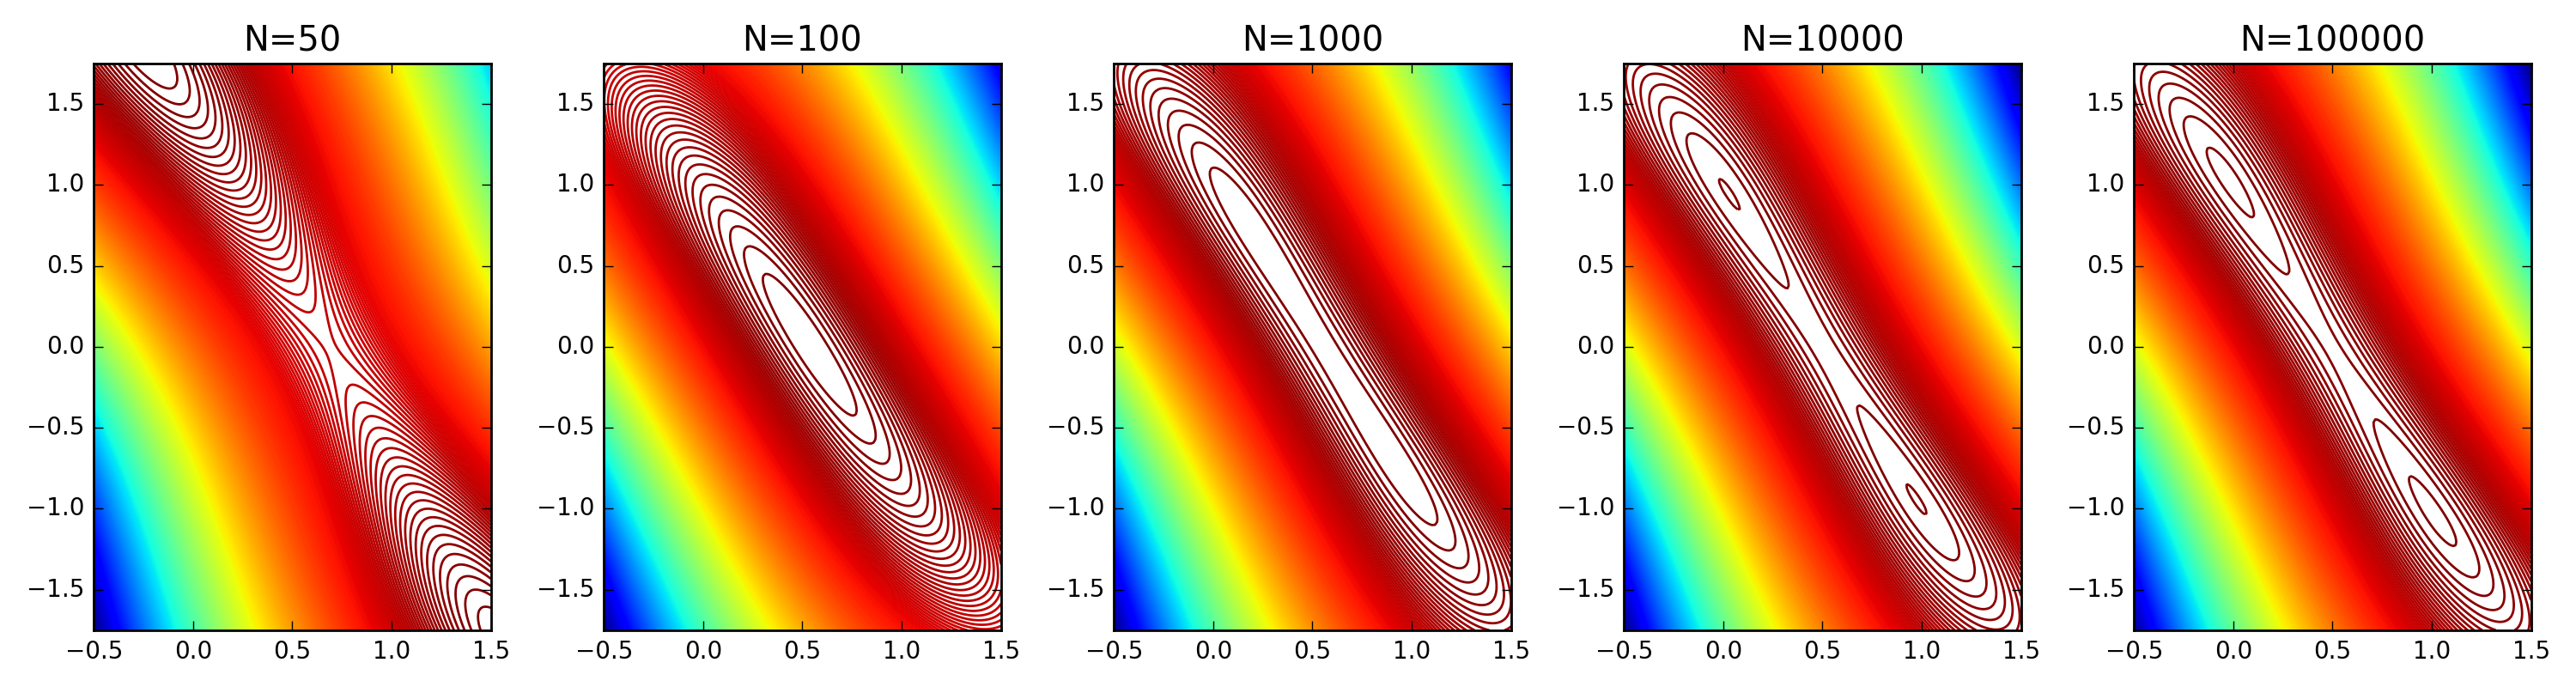
\includegraphics[width=1\linewidth]{contour_v1}
  \caption{The posterior distribution, from 50 to 100k samples, with temperature set at 1.}
  \label{fig:contour1}
\end{figure}
\begin{figure}[t]
  \centering
  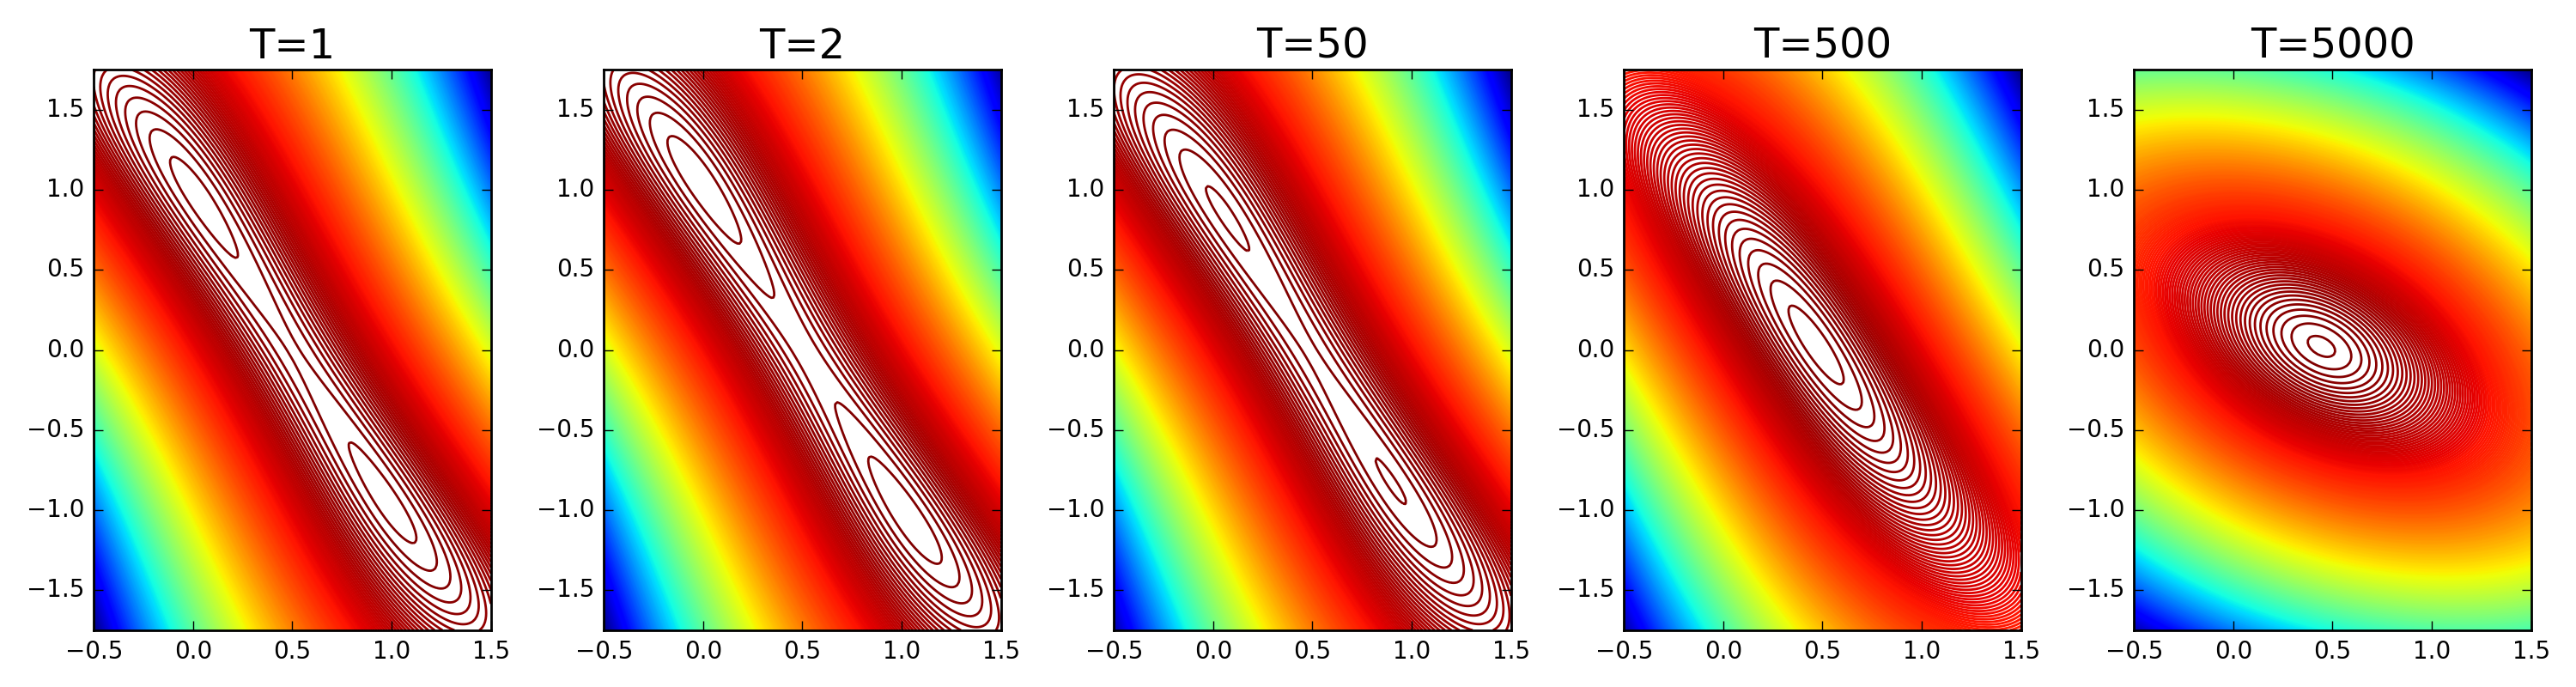
\includegraphics[width=1\linewidth]{contour_v2}
  \caption{The posterior distribution, with $N=10000$ but with temperature $T$ varying.}
  \label{fig:contour2}
\end{figure}

To gain some intuition on what the posterior looks like, Figure~\ref{fig:contour1} shows simulated
contour plots of the posterior based on varying numbers of data points $N$, with the temperature set
at $T=1$. Note that because we are using all $N$ points here, the scale factor $N/n=1$. As $N$
increases, the posterior converges to a multimodal distribution with modes at $(0,1)$ and $(1,-1)$.
Figure~\ref{fig:contour2} is similar, except this time we fix the number of samples at $N=10000$,
but show how changing the temperature $T$ affects the distribution. A larger $T$ implies a flatter
posterior, one that (weakly) peaks in between the two true modes.


\section{Logistic Regression Experiment Details}\label{app:logistic}

In this section, we go over some details of our logistic regression experiment. The feature vector
for an image consists of its pixel values, normalized between 0 and 1. For simplicity, we only
consider the binary classification case, so we only use digits one (denoted as output $y = 1$) and
seven (denoted as $y = -1$). The probability of the $i^{\rm th}$ output $y_i \in \{-1,+1\}$ with the
input vector $x_i$ is
\begin{equation}
p(y_i \mid x_i) = \frac{1}{1+\exp (-y_i \theta^T x_i)},
\end{equation}
where $\theta$ is the 784-length parameter vector.

For our experiment, we impose a uniform prior to represent our lack of knowledge about $\theta$.  We
use a random walk proposer, which can be modeled as $\theta' = \theta_i + \mathcal{N}(0,
\sigma^2I)$, where $\theta_i$ is the current sample, $\theta'$ is the proposed sample, and we choose
the variance to be a constant $\sigma^2 = 0.01$ for all components. We initialize $\theta_0$ to be a
vector of all ones, and set our minibatch size as $m=50$.

For our minibatch MH test, in order to enforce the ${\rm std}(\Delta') < 1.2$ condition, we use a
constant temperature $T = 3000$. If our estimated ${\rm std}(\Delta') \ge 1.2$, we ignore the
current iteration.  Figure~\ref{fig:appendixExp2} plots our estimated ${\rm std}(\Delta')$ values
versus iteration count. 

\begin{figure}[t]
  \centering
  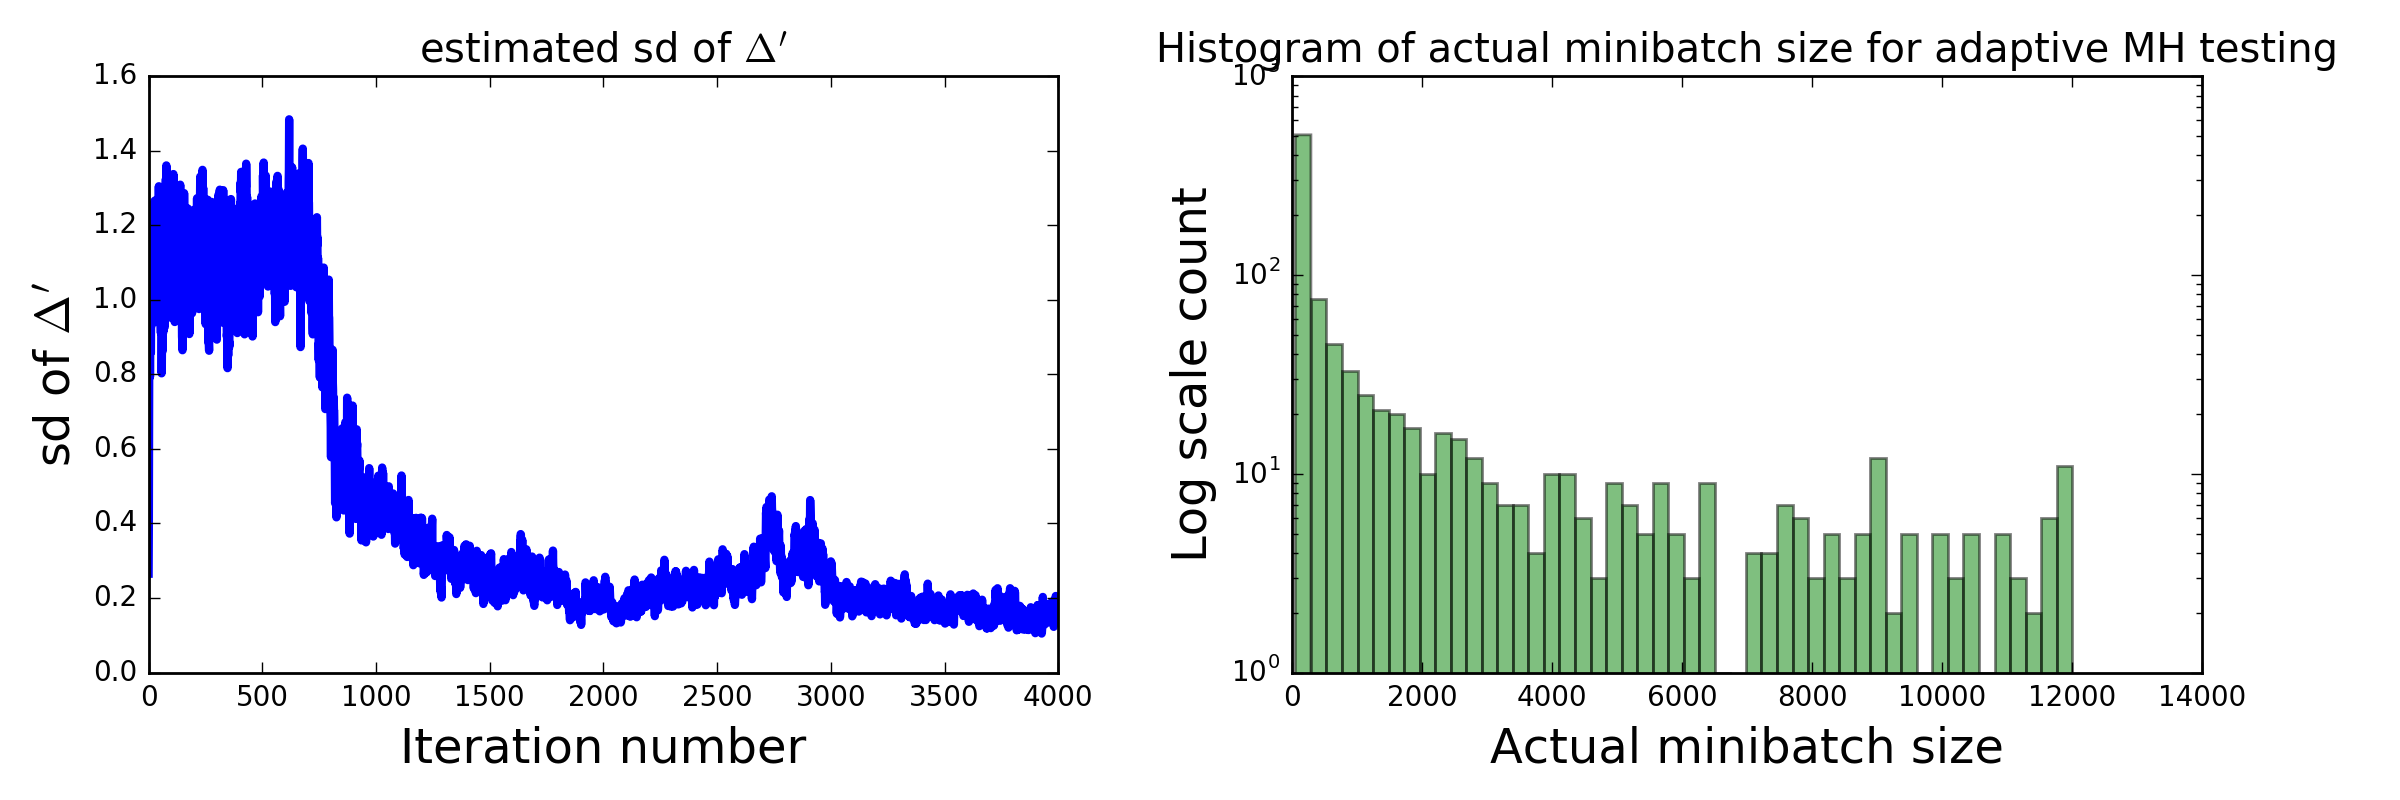
\includegraphics[width=1\linewidth]{./figures/appendixExp2}
  \caption{Additional results for the logistic regression experiment.}
  \label{fig:appendixExp2}
\end{figure}

For adaptive MH testing, our experimental settings are the same as with our MH test, except we do
not impose a temperature. The minibatch size of adaptive MH testing is also initialized as 50, but
it may increase by that amount each iteration. Figure~\ref{fig:appendixExp2} shows the histogram of
the actual minibatch size at the end of each iteration in adaptive MH testing.


\section{Neural Network Experiment Details}\label{app:nnet}

For our neural network experiment, we use the architecture discussed in Section~\ref{ssec:nets}. We
use the SGHMC as the proposer for our minibatch MH testing. For the baseline, we use a tuned
adaptive gradient descent optimizer, whose step size changes by $0.01 /(i+1)^{0.4}$. Both methods
have minibatch sizes set at $m=200$. There are one million total data instances $x_i$.

For SGHMC, we use the simplified update equations~\cite{sghmc_2014}:
\begin{equation}
\Delta \theta = v, \quad \quad\Delta v = -\eta \nabla U(\theta) - \alpha v + \mathcal{N}(0, 2(\alpha
-\hat{\beta}) \eta),
\end{equation}
where $v$ represents auxiliary momentum variables, and $\nabla U(\theta)$ is the gradient of the
system. We set the hyperparameters to be $\eta_i = 0.01 /(i+1)^{0.4}$, and $\alpha=0.1$. We use the
empirical Fisher~\cite{conf/icml/AhnBW12} information $V(\theta)$ to estimate the value of
$\hat{\beta}$, so that $\hat{\beta}=\frac{1}{2}\eta V(\theta)$. In order to control ${\rm
std}(\Delta')$, we initialize the temperature at 1000, and adjust it at iteration $i$ according to
$T_i = \max\{1, 1000/(i+1)^{0.5}\}$.

% Daniel: here are example LaTeX codes for figures and tables if we want to use them.
%\begin{figure}[h]
%  \centering
%  \fbox{\rule[-.5cm]{0cm}{4cm} \rule[-.5cm]{4cm}{0cm}}
%  \caption{Sample figure caption.}
%\end{figure}
%\begin{table}[t]
%  \caption{Sample table title}
%  \label{sample-table}
%  \centering
%  \begin{tabular}{lll}
%    \toprule
%    \multicolumn{2}{c}{Part}                   \\
%    \cmidrule{1-2}
%    Name     & Description     & Size ($\mu$m) \\
%    \midrule
%    Dendrite & Input terminal  & $\sim$100     \\
%    Axon     & Output terminal & $\sim$10      \\
%    Soma     & Cell body       & up to $10^6$  \\
%    \bottomrule
%  \end{tabular}
%\end{table}
%\usepackage[pdftex]{graphicx} ...
%\includegraphics[width=0.8\linewidth]{myfile.pdf}

\end{document}

